\chapter{Implementation of a Prototype}\label{chap:prototype}

This chapter describes the implementation of the prototype created to test the viability of Replico. It begins by explaining the architecture, hardware, software, and tools used to develop the prototype. The chapter then details how hand detection is performed, the various states within the system, how tables are tracked, how finger input is interpreted, the methods for displaying feedback to users, and the networking implementation details.

\section{Architecture}
    
    To develop the prototype, two HTC Vive Pro 2 headsets and two multi-touch surfaces -- a 32-inch infrared frame and a 47-inch capacitive Displax Skin Ultra\footnote{\url{https://www.displax.com/skin-ultra} } touchscreen -- were used. The Unity\footnote{\url{https://unity.com/}} game engine was chosen for its robust VR support, personal previous experience, extensive community resources, and excellent compatibility with external C\# libraries, which helped reduce development risks.
    
    Unity's OpenXR plugin\footnote{\url{https://docs.unity3d.com/Packages/com.unity.xr.openxr@1.11/manual/index.html}} controls VR hardware communication, handling input and rendering with minimal effort, and managing all API calls automatically. OpenXR\footnote{\url{https://registry.khronos.org/OpenXR/specs/1.1/html/xrspec.html}} is an API standard developed by Khronos for XR applications, including VR, and is widely adopted across many XR devices with conformant runtimes. Due to its ubiquity and recency, it was chosen over alternatives such as using SteamVR directly.

    Since Unity's OpenXR plugin interfaces with Unity's Input System, the Unity Enhanced Touch API\footnote{\url{https://docs.unity3d.com/Packages/com.unity.inputsystem@1.0/api/UnityEngine.InputSystem.EnhancedTouch.html}} was used instead of the standard Unity Touch API to maintain a consistent input management system. The Enhanced Touch API provides automatic finger tracking and keeps a history of touch interactions.

    The first-party Unity Netcode for GameObjects\footnote{\url{https://docs-multiplayer.unity3d.com/netcode/current/about/}} library was used for networking. This library offers a straightforward abstraction of networking logic and is easy to use and set up for client-server or distributed authority topologies. Its simplicity is well-suited for a small number of clients, making it ideal for this prototype.


    \begin{figure}[h]
        \centering
        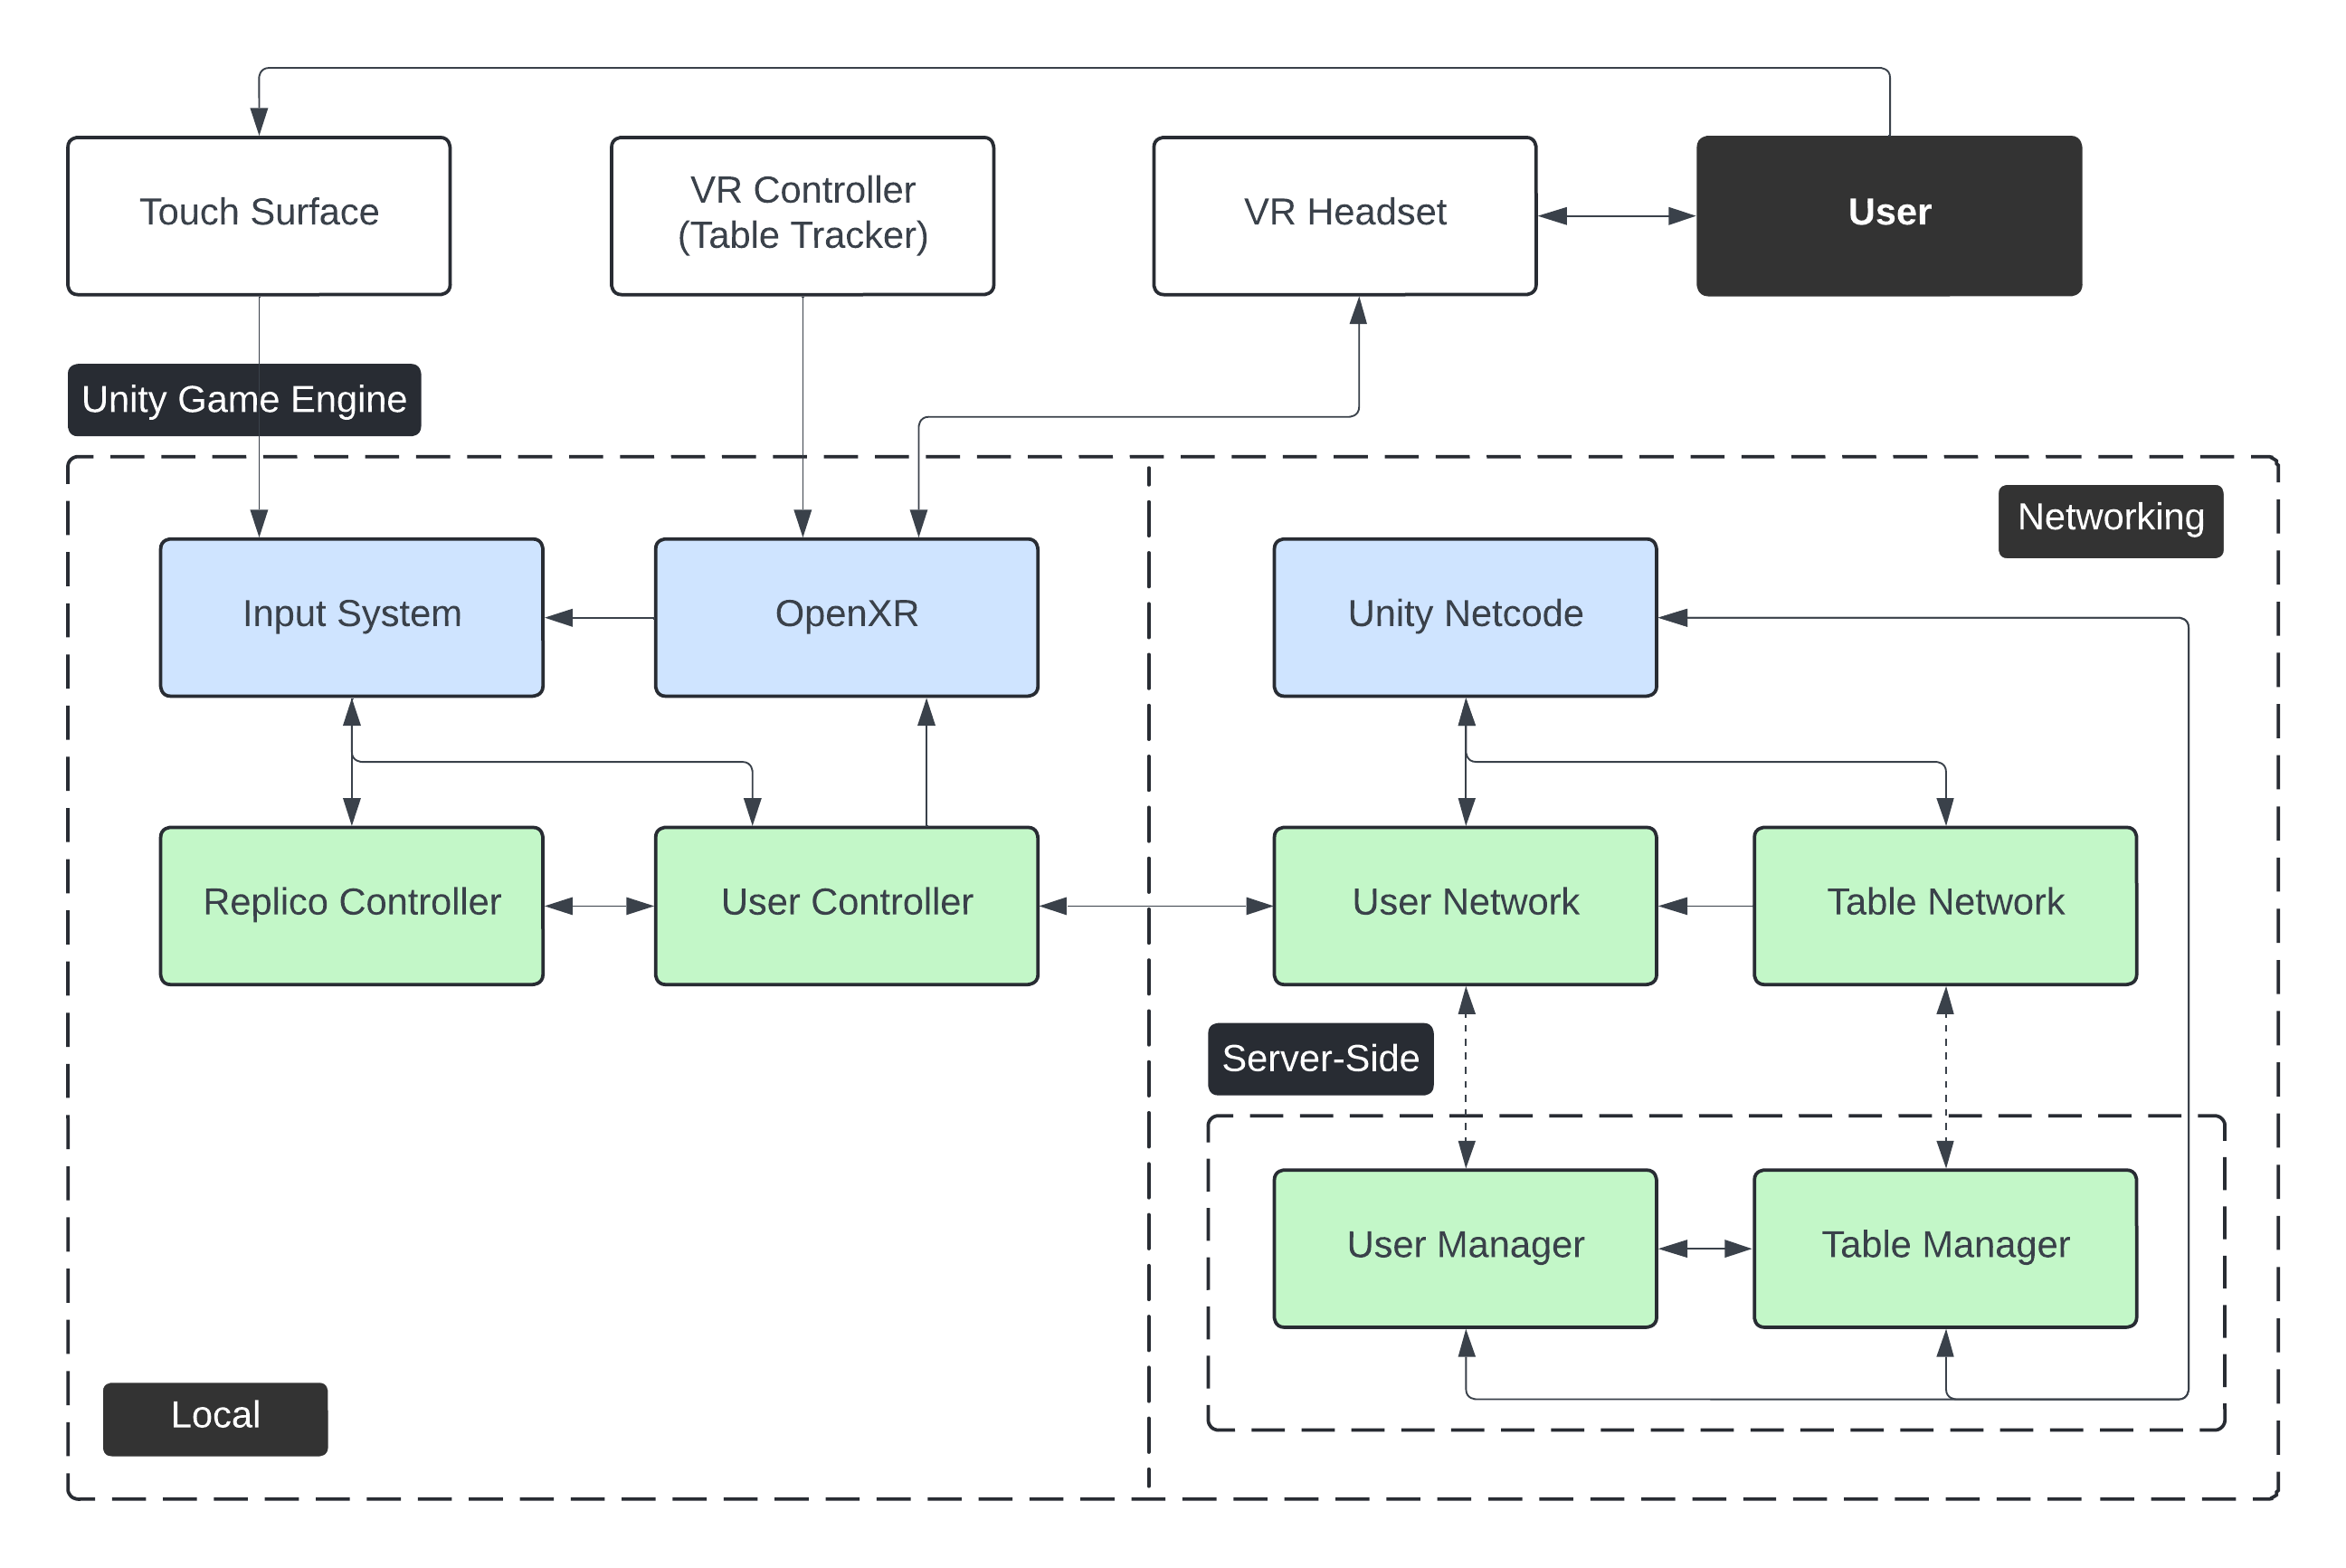
\includegraphics[width=.97\linewidth]{figures/architecture.png}
        \caption{System architecture. Modules in blue represent Unity libraries, while the prototype implements modules in green.}
        \label{fig:architecture}
    \end{figure}
    
    The system architecture diagram in Figure \ref{fig:architecture} demonstrates the integration of various software and hardware components, describing both local and networked elements. OpenXR manages communication with the VR headset and the table tracker, rendering images to the headset, updating the virtual camera's position, and interfacing inputs to Unity's Input System. Unity's Enhanced Touch API processes touches sensed by the touch surface. The Replico Controller and User Controller manage interaction logic and user actions, communicating with the Input System and OpenXR. Networking is handled by Unity Netcode, which synchronizes user and table data across the network via the User Network and Table Network, using a client-server topology. The server-side User Manager and Table Manager manage data for users and tables. The User Manager tracks users in the system and communicates with the User Network objects through remote procedure calls (RPCs) and network variables. The Table Manager handles table creation, deletion, and management logic, communicating with Table Network objects using RPCs and network variables.


        % city
        % rover and ground textures
        % dungeon assets and the modular asset builder tool (https://fertile-soil-productions.itch.io/mast)

\section{State Machine}

    The interpretation of touch surface input varies depending on the gestures employed. To address this, a state machine was created. A state machine consists of defined states with distinct transitions, where each state processes the input differently. The implementation was done through the state design pattern, wherein each step is represented as a class that alters the behavior of the Replico controller. Figure \ref{fig:states} provides a diagram illustrating the implemented state machine.

    \begin{figure}[h]
        \centering
        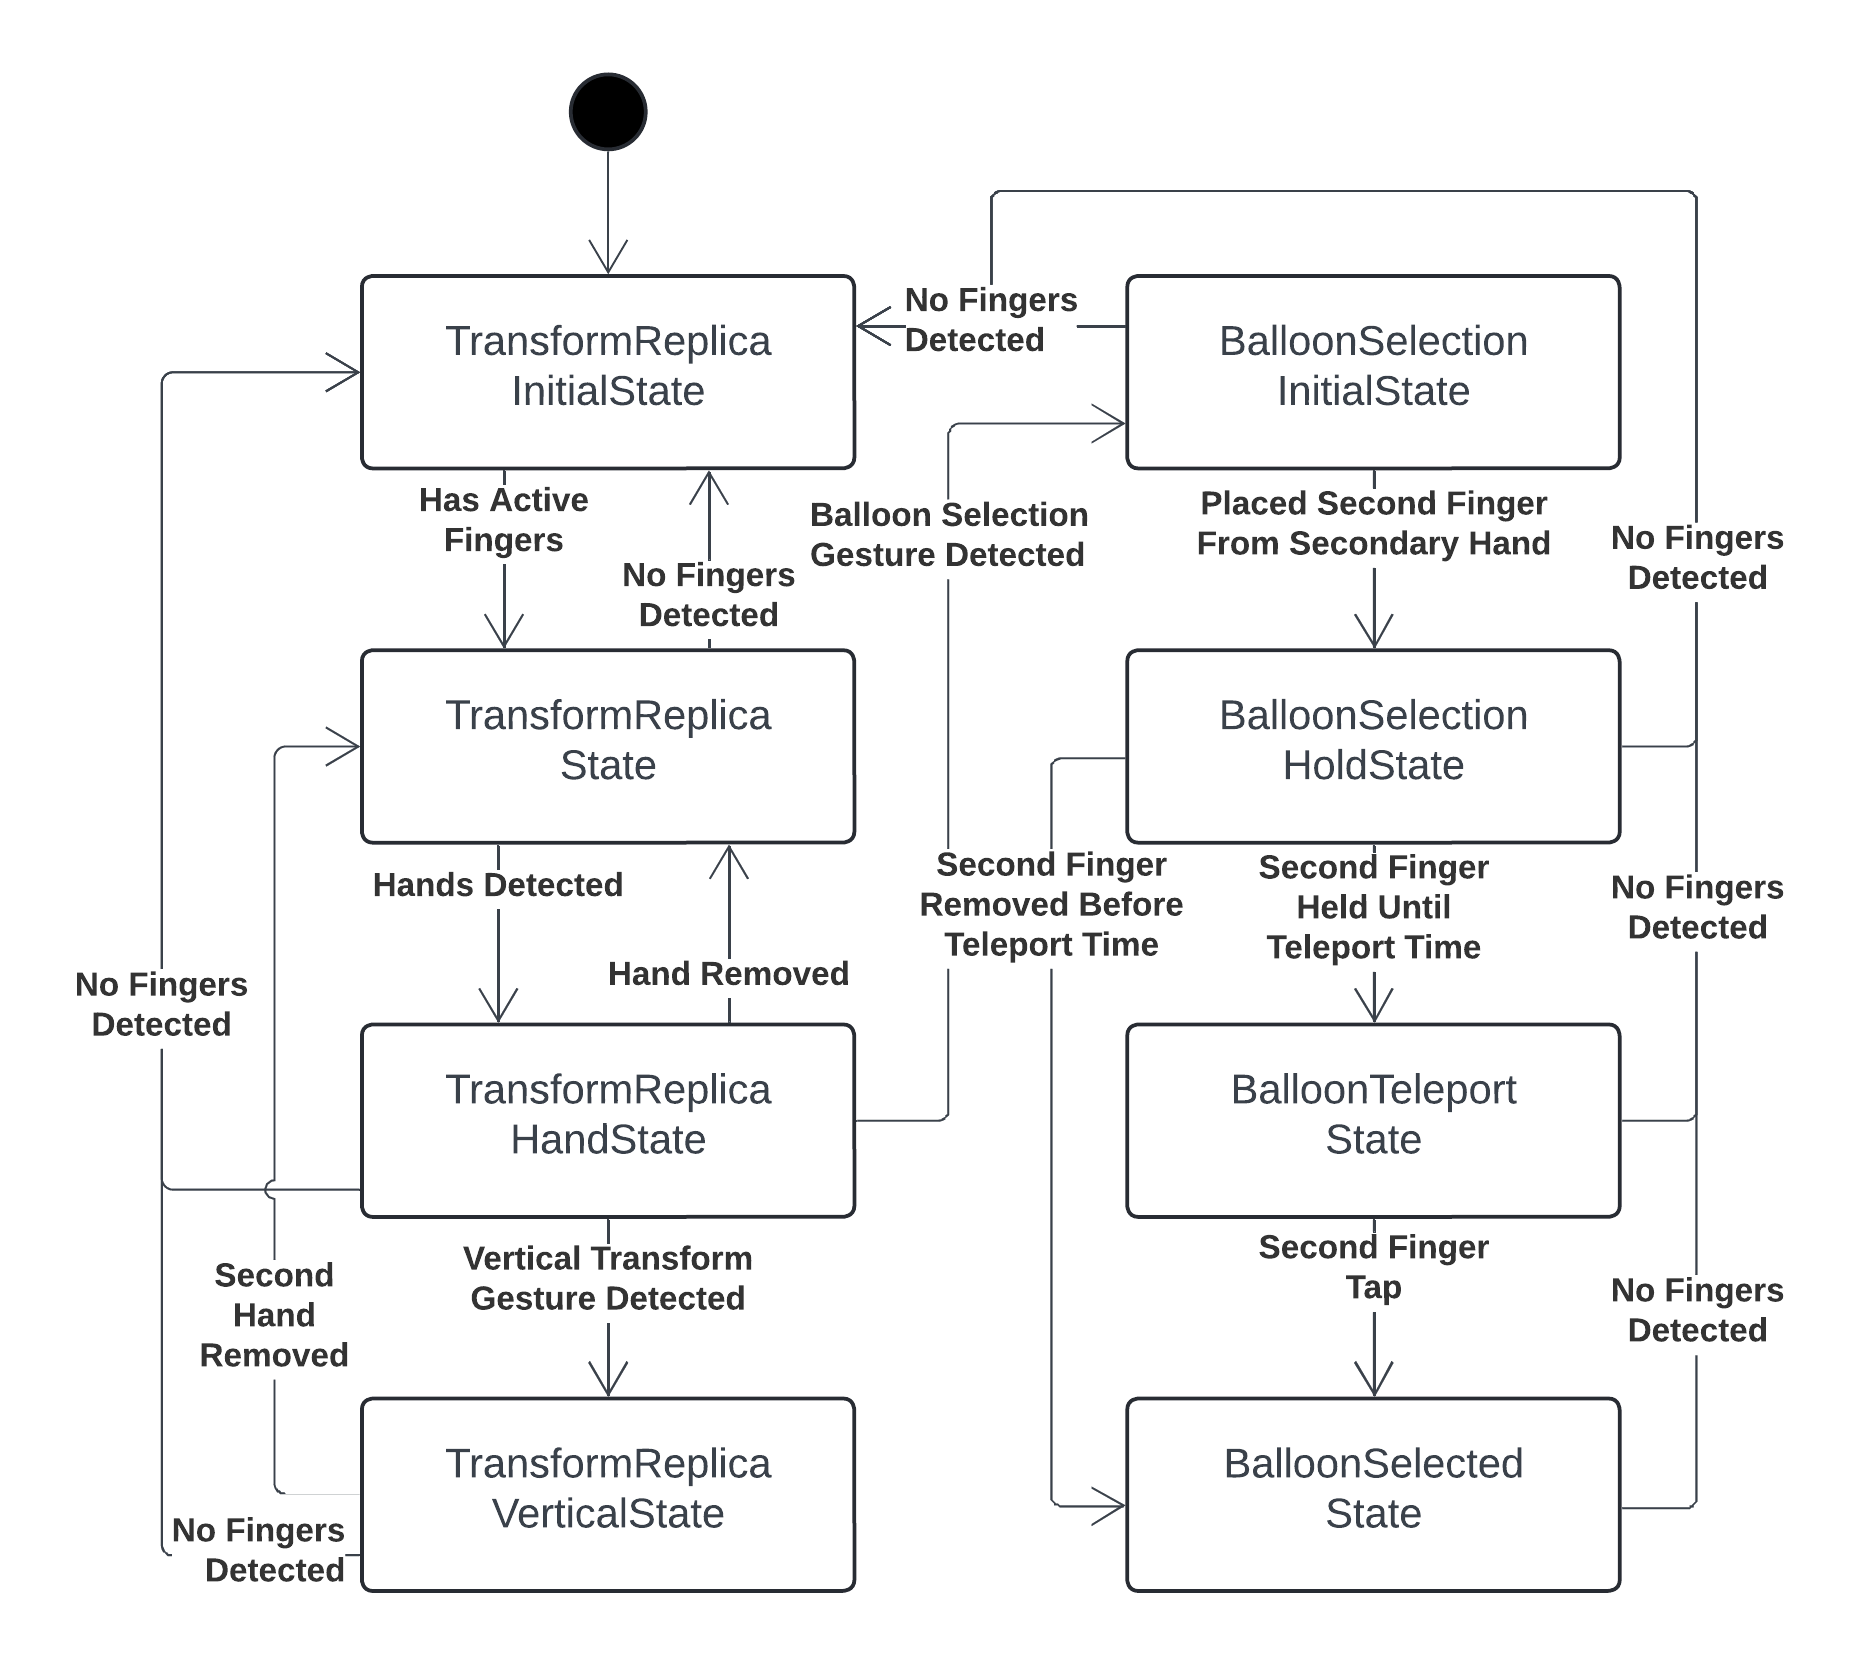
\includegraphics[width=1\linewidth]{figures/states.png}
        \caption{State machine diagram.}
        \label{fig:states}
    \end{figure}

    The \lstinline{TransformReplicaInitialState} is the starting state where no fingers are detected, and therefore no controls are active. In this state, finger touches are checked every frame using the Enhanced Touch API, which updates every frame because the Input System update mode is set to Dynamic. When at least one finger is detected, the system transitions to \lstinline{TransformReplicaState}. All states revert to this initial state whenever no fingers are detected.
    
    The \lstinline{TransformReplicaState} is entered when fingers are detected, but no hands are recognized yet. In this state, the user can move the replica using the gestures described in Section \ref{sec:transform} and implemented in Section \ref{sec:transformation}. This state performs hand detetction using the method described in Section \ref{sec:hand}, every frame. When both hands are detected, it transitions to \lstinline{TransformReplicaHand}\lstinline{State}.
    
    In \lstinline{TransformReplicaHandState}, users can move the replica as in \lstinline{TransformReplica}\lstinline{State}. This state checks what gesture the user is doing in every frame using the method described in Section \ref{sec:vertical_balloon}. It transitions to \lstinline{TransformReplicaVerticalState} if the vertical transform gesture is detected, or to \lstinline{BalloonSelectionInitialState} if the balloon selection gesture is detected. If any hand is removed, it transitions back to \lstinline{TransformReplicaState}.

    In \lstinline{TransformReplicaVerticalState}, the user can move the replica as in \lstinline{TransformReplica}\lstinline{State} using their primary hand, while the secondary hand performs translation on the XY plane. To allow users to temporarily remove the secondary hand to reposition their fingers without terminating the gesture, the secondary hand may be removed for up to $0.55$ seconds before the controller transitions back to \lstinline{TransformReplicaState}.

    In \lstinline{BalloonSelectionInitialState}, the user performs the balloon selection gesture as described in Section \ref{sec:balloon}. The primary finger moves the balloon on the XZ plane, while moving the fingers together raises the balloon and moving them apart lowers it. The balloon's height is saved between gestures, so the user doesn't have to raise it each time they start balloon selection. It transitions to \lstinline{BalloonSelectionHoldState} when a second finger is added to the secondary hand. Instead of transitioning instantly to the initial state when no fingers are detected, there is a grace period of $0.15$ seconds. This grace period accounts for potential hardware tracking failures that could prematurely stop the balloon selection gesture, potentially causing frustration.

    The \lstinline{BalloonSelectionHoldState} monitors how long the user holds down the second finger from the secondary hand. If the finger is held for $0.4$ seconds or the primary hand moves, the state transitions to \lstinline{BalloonTeleportState}. Removing the finger before $0.4$ seconds results in different actions: joining a table if the balloon intersects one, acknowledging or deleting a point of interest if it intersects one, or creating a new point of interest if it intersects none, thereby transitioning to \lstinline{BalloonSelectedState}.

    In \lstinline{BalloonTeleportState}, the user can rotate their balloon using the same gesture as rotating the replica, following the calculations described in \ref{sec:transformation}. Confirmation of teleportation occurs if the user taps with the second finger of their second hand (removing and placing it again) or if two touches are detected within the hand detection distance outlined in \ref{sec:hand}. Upon confirmation, the controller transitions to \lstinline{BalloonSelectedState}.
    
    The purpose of \lstinline{BalloonSelectedState} is to act as a buffer between balloon selection interactions and replica transformations. Users can only perform replica transformations after removing all finger touches, at which point the controller transitions back to \lstinline{TransformReplicaInitial}\lstinline{State}.


\section{Replica Transformations} \label{sec:transformation}

    This section discusses the transformations applied to the replica in states \lstinline{TransformReplicaState}, \lstinline{TransformReplicaHandState}, and \lstinline{TransformReplicaVerticalState}.
    
    Translation is achieved by calculating the distance \(\vec{D} = C_{i} - C_{i-1}\), where \(C_{i}\) and \(C_{i-1}\) are the centers of the active touches on the touch surface from the current frame and the previous frame, respectively, as shown in Equation \ref{eq:center}.

    \begin{figure}[h]
    \begin{equation}
    \begin{split} \label{eq:center}
        \mathbf{F}_i &= \{(x_{i_k}, y_{i_k}) :\ k = 1,\ \dots,\ n\} \\
        \mathbf{minF}_i &= (\min_{k} x_{i_k},\ \min_{k} y_{i_k}) \\
        \mathbf{maxF}_i &= (\max_{k} x_{i_k},\ \max_{k} y_{i_k}) \\
        C_i &= \frac{\mathbf{minF}_i + \mathbf{maxF}_i}{2}
    \end{split}
    \end{equation}
    \end{figure}

    Here, \(\mathbf{F}_i\) represents the positions of the \(n\) fingers in the \(i\)-th frame, \(\mathbf{minF}_i\) and \(\mathbf{maxF}_i\) are the minimum and maximum x and y coordinates from the set of finger positions. Essentially, \(C_i\) is the geometric centroid of the smallest rectangle that can enclose all the touch points. The distance $\vec{D}$ is then multiplied by a factor \(t\), which can be adjusted for each 3D model, resulting in \(\vec{T} = t \cdot \vec{D}\). This yields a 2D vector that is added to the replica's position in the \(XZ\) plane.

    Scaling is achieved by first calculating $s = {{\left(\bar{d_i} / \bar{d_{i-1}}\right)}^{c}}$, where \(\bar{d_i}\) and \(\bar{d_{i-1}}\) are the average distances of the active touches to the center of those touches from the current frame and the previous frame, respectively, and \(c\) is a constant used to modulate the scaling effect. The calculation for the average distance is shown in Equation \ref{eq:distance}.
    
    \begin{figure}[h]
    \begin{equation}
    \begin{split} \label{eq:distance}
        \bar{d_i} &= \frac{\sum_{k = 1}^{n} \| C_i - F_{i_k} \|}{n}
    \end{split}
    \end{equation}
    \end{figure}
    
    Finally, this scaling is applied to the replica around a base point, based on the center of the fingers. To do this, the pivot point in world coordinates, \(\mathrm{pivot}_w\), is first converted to local coordinates, \(\mathrm{pivot}_l\), relative to the replica. The replica's local scale is then multiplied by \(s\). After scaling, the position of the pivot in world coordinates, \(\mathrm{pivot}_k\), calculated by converting \(\mathrm{pivot}_l\) back to world coordinates, will not be equal to \(\mathrm{pivot}_w\). To correct this, the displacement \(\vec{\Delta \mathrm{pivot}} = \mathrm{pivot}_w - \mathrm{pivot}_k\) is calculated and added to the replica's world position.

    Rotation is achieved by calculating the fingers' average rotation \(\bar{\theta}\). The calculation for this is shown in Equation \ref{eq:rotation}, where \(\vec{\mathrm{dir}_{i_k}}\) is the vector direction from the center of the fingers to the \(k\)-th finger in the \(i\)-th frame, \(|\theta_k|\) is the angle between the vector direction of the previous frame and the current frame for the \(k\)-th finger. The angle \(\theta_k\) is determined by adjusting \(|\theta_k|\) based on the cross product's \(z\)-component to account for direction, as the arccosine function's range only goes from \(0\) to \(\pi\). The replica is then rotated around the \(Y\) axis that passes through \((C_{i_x}, 0, C_{i_y})\) with the angle $\bar{\theta}$, using Unity's \lstinline{RotateAround}.

    \begin{equation}
    \begin{split} \label{eq:rotation}
        \vec{\mathrm{dir}_{i_k}} &= \mathbf{F}_{i_k} - C_i \\
        |\theta_k| &= \cos^{-1} \left( \frac{\vec{\mathrm{dir}_{{i-1}_k}} \cdot \vec{\mathrm{dir}_{i_k}}}{\|\vec{\mathrm{dir}_{{i-1}_k}}\| \|\vec{\mathrm{dir}_{i_k}}\|} \right) \\
        \theta_k &= \begin{cases} 
            |\theta_k| & \text{if} \quad (\vec{\mathrm{dir}_{{i-1}_k}} \times \vec{\mathrm{dir}_{i_k}})_z < 0 \\
            -|\theta_k| & \text{if} \quad (\vec{\mathrm{dir}_{{i-1}_k}} \times \vec{\mathrm{dir}_{i_k}})_z \geq 0
        \end{cases} \\
        \bar{\theta} &= \frac{\sum_{k=1}^{n} \theta_k}{n}
    \end{split}
    \end{equation}


    In the \lstinline{TransformReplicaVerticalState}, the primary hand can perform $XZ$ translation, rotation, and scaling, while the secondary hand can only perform translation on the $XY$ plane. Only the fingers from the primary hand are considered for transformations with the primary hand. The secondary hand's fingers can only perform translation as previously described, but instead of \(\vec{T}\) being applied to the replica's $XZ$ position, it is applied to the $XY$ position.
    
    The transformations are not directly applied to the replica; instead, they are applied to a target object. The replica then follows this target object using Unity's \lstinline{SmoothDamp} for position and scale, and \lstinline{SmoothDampAngle} for each Euler rotation angle. This helps to reduce jitter caused by low-frequency or low-accuracy touch input updates.

\section{Gesture Detection}

    This section explains how the different gestures -- transformation, vertical transformation, and balloon selection -- are distinguished. Section \ref{sec:hand} explains the method for detecting and distinguishing the user's hands, and Section \ref{sec:vertical_balloon} describes how the vertical transform and balloon selection gestures are differentiated.

    \subsection{Hand Detection} \label{sec:hand}

        Detection and distinction of hands are important for recognizing Replico's touch-based gestures. The prototype took a simplistic approach to hand detection, using input solely from the touch surface and Unity's Enhanced Touch API. The method involves detecting two clusters based on finger proximity. For this purpose, this prototype uses a naive K-Means clustering algorithm \cite{zbMATH03340881, lloydLeastSquaresQuantization1982, 1571980074621944832} with a $k$ value of $2$. The algorithm was implemented using the ML.NET library\footnote{\url{https://github.com/dotnet/machinelearning}}, a machine learning library for .NET. For compatibility with Unity, the .NET Standard 2.1 version was used. The distance function used is the Euclidean distance between the finger positions on the touch surface in pixels, 
        and the Yinyang initialization algorithm \cite{pmlr-v37-ding15} is applied.
    
        Other clustering algorithms, such as DBSCAN \cite{ester1996density}, were not used because they do not allow the specification of a fixed number of clusters ($k$) or because they perform better with a larger number of clusters. K-means is perfectly adequate in this case with a maximum of $10$ points (one for each finger) and only $2$ clusters.
    
        The K-means algorithm returns two clusters of fingers when more than one finger is placed on the touch surface. However, this can result in two fingers from the same hand being detected as separate clusters. To address this, a distance threshold between cluster centroids is used to determine if the clusters represent separate hands. The threshold distance is measured relative to a min-max normalized value of the screen dimensions in pixels. A distance threshold of $0.18$ was found to be effective through testing.
    
        Initially, before any hands have been detected in the \lstinline{TransformReplicaState} shown in Figure \ref{fig:states}, the distinction between the primary and secondary hands is maintained by queuing fingers based on the order of their touch. The cluster containing the first detected finger represents the primary hand. Once both hands are detected in the \lstinline{TransformReplicaHandState} and beyond, hands are updated each frame by reapplying the K-means algorithm. The distinction is then made by counting how many fingers from the previously detected primary hand are in each newly detected cluster; the cluster with the most fingers from the primary hand is associated with it. To update the hands, new fingers in the clusters are added to the corresponding hands, and previously detected fingers remain in their respective hands unless they have been removed from the touch surface. This approach allows left-handed and right-handed users to perform all Replico gestures easily.

    \subsection{Distinguishing Vertical Transform and Balloon Selection} \label{sec:vertical_balloon}
    
        The vertical transform and balloon selection gestures, described in Sections \ref{sec:transform} and \ref{sec:balloon} respectively, can be easily confused with the pinch gesture required for scaling the replica. To aid in this distinction:
    
        \begin{itemize}
            \item \textbf{Vertical Transform:} At least one finger on the primary hand and at least two fingers on the secondary hand. The secondary hand must remain stationary for $0.2$ seconds.
            \item \textbf{Balloon Selection:} Exactly one finger on the primary hand and exactly one finger on the secondary hand. Both hands must remain stationary for $0.2$ seconds.
        \end{itemize}
    
        The vertical transform only checks if the second hand has moved, allowing the user to add the secondary hand while transforming with the first. The criterion for determining if a hand hasn't moved is that none of its fingers have moved past a threshold $\delta$ from the position where they were first placed. This threshold is measured relative to a min-max normalized value of the screen dimensions in pixels, with testing indicating $0.01$ as an appropriate value. Once a finger has moved, it will be considered moved until it is removed.

\section{Table Tracking} \label{sec:table_tracking}

    The user's table is tracked to a real-world table using a VR controller, as shown in Figure \ref{fig:table_tracking}. The controller is positioned pointing toward the user instead of forward from the table so that the tracked controller position matches the table's corner. If it pointed the other way, a translation based on the controller's length toward the table corner would be necessary, which is not feasible for all controller types.

    \begin{figure}[h]
        \centering
        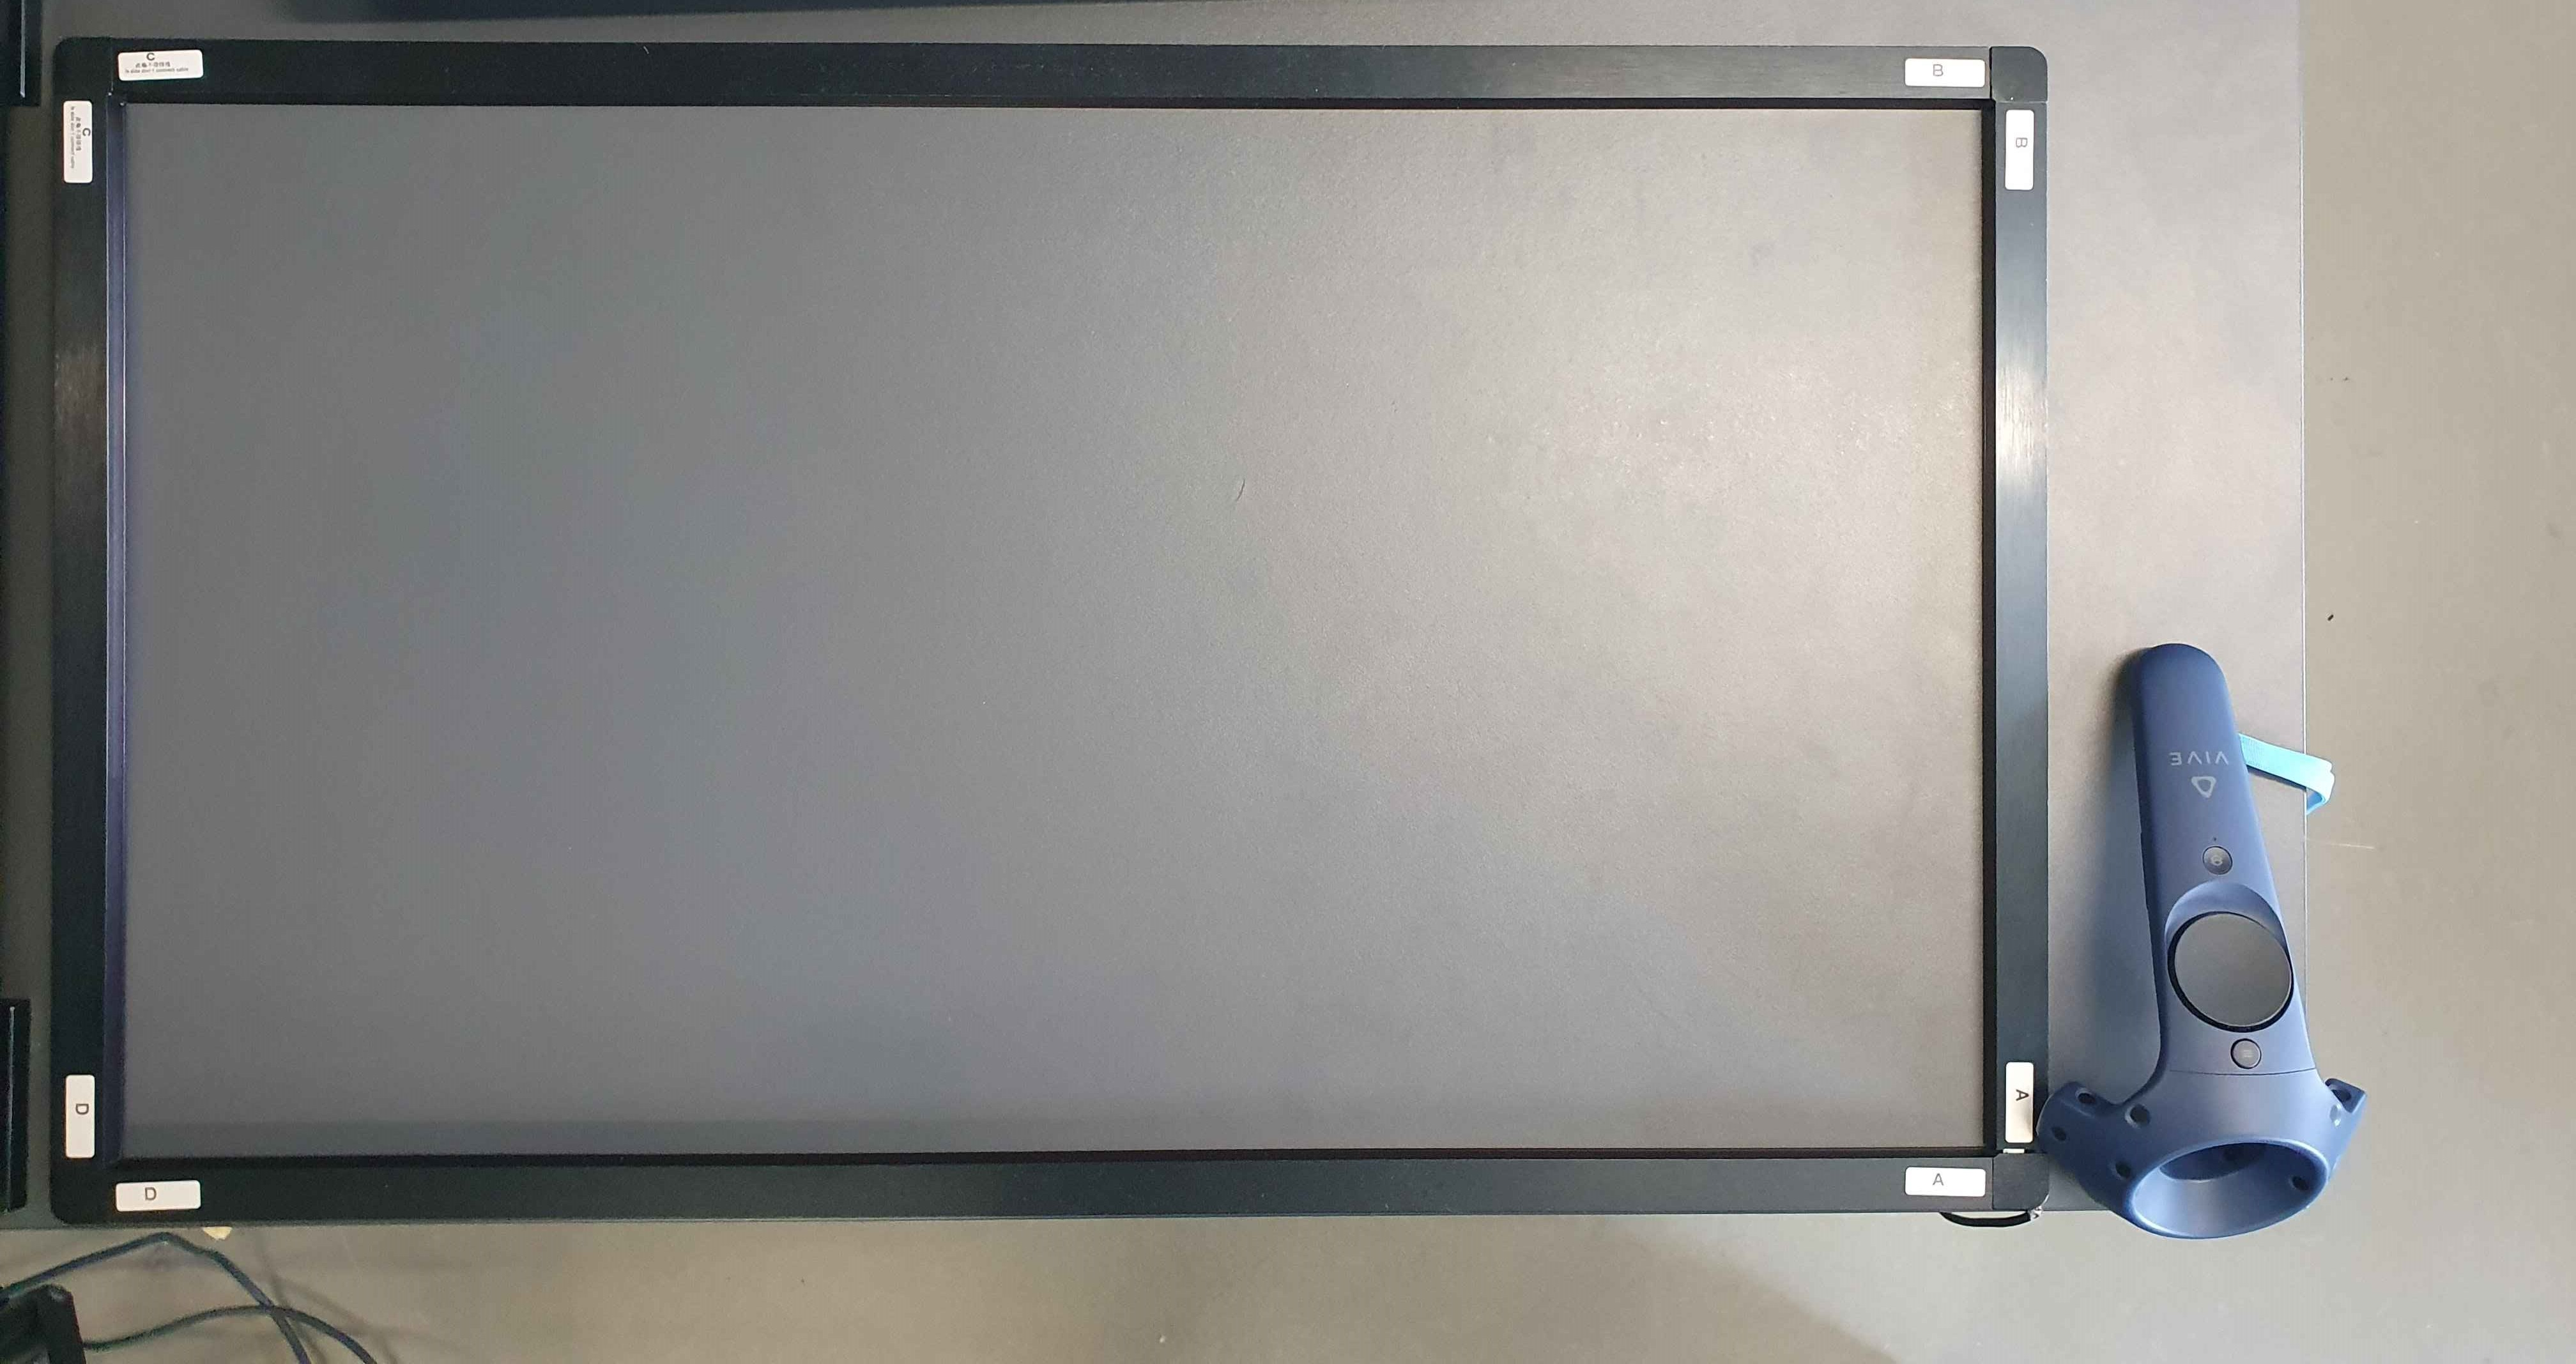
\includegraphics[width=1\textwidth]{figures/table_tracking.jpg}
        \captionof{figure}{Tracking the table using a VR controller.}
        \label{fig:table_tracking}
    \end{figure}

    When attaching a user to a virtual table, such as when the user joins a table or teleports, the orientation and position of the tracker must match the orientation and position of the table's attach point, which is an empty GameObject on the table's Prefab. To achieve this, the user's orientation is first updated using \lstinline{MatchOriginUpCameraForward}, followed by updating the position with \lstinline{MoveCameraToWorldLocation}, both functions from the OpenXR plugin. 

    The \lstinline{MatchOriginUpCameraForward} function requires two parameters: an up vector and a forward vector. The up vector is set to match the attach point's up vector, assuming the user and controller are on flat ground. The forward vector, \(\vec{v}_{\mathrm{forward}}\), is calculated as shown in Equation \ref{eq:tracker}. Here, $\mathbf{q}_{\mathrm{tracker}}$ represents the quaternion rotation of the tracker, and $\mathbf{q}_{\mathrm{attach}}$ represents the quaternion rotation of the table's attach point. $\Delta\theta$ is the rotation of the attach point relative to the tracker. The yaw component is isolated to ignore pitch and roll, preventing rotation along the x and z axes due to the controller rolling, assuming the user is on flat ground. $\mathbf{q}_{\mathrm{target}}$ is the user's target rotation, combining the user's current yaw rotation with the relative rotation of the attachment point. Finally, the forward vector is obtained by multiplying $\mathbf{q}_{\mathrm{target}}$ by the (0,0,1) vector. The \lstinline{MoveCameraToWorldLocation} function requires a position parameter. This position is calculated using the equation $P = P_{\mathrm{attach}} + P_{\mathrm{user}} - P_{\mathrm{tracker}}$.

    \begin{figure}[h]
    \begin{equation}
    \begin{split} \label{eq:tracker}
        \Delta\theta&=\mathbf{q}_{\mathrm{tracker}}^{-1}\cdot \mathbf{q}_{\mathrm{attach}} \\
        \Delta\theta_Y &= \mathrm{Quat}\left(0, \mathrm{yaw}(\Delta\theta), 0\right) \\
        \mathbf{q}_{\mathrm{user}_Y} &= \mathrm{Quat}(0, \mathrm{yaw}(\mathbf{q}_{\mathrm{user}}), 0) \\
        \mathbf{q}_{\mathrm{target}} &= \mathbf{q}_{\mathrm{user}_Y} \cdot \Delta\theta_Y \\
        \vec{v}_{\mathrm{forward}} &= \mathbf{q}_{\mathrm{target}} \cdot (0,0,1)
    \end{split}
    \end{equation}
    \end{figure}

    Because the controller may fall accidentally while the user is interacting with the touch surface and cannot see it when using the VR headset, it is only used to track the table when the user first joins a table. To achieve this, the tracker's rotation relative to the user is calculated using $\mathbf{q}_{\mathrm{local}} = \mathbf{q}_{\mathrm{tracker}} \cdot \mathbf{q}_{\mathrm{user}}^{-1}$ and stored. Additionally, the tracker's local position relative to the user is calculated using the user's \lstinline{InverseTransformPoint} function and stored.

    To convert the local rotation back to world rotation, the calculation  $\mathbf{q}_{\mathrm{tracker}} = \mathbf{q}_{\mathrm{user}} \cdot \mathbf{q}_{\mathrm{local}}$ is used. Similarly, the local position is converted back to world position utilizing the user's \lstinline{TransformPoint} function. These world coordinates and rotations are then used in the previously described calculations.

\section{Visual Feedback}

    The prototype uses various visual indicators as forms of feedback. These include a virtual touch frame with finger indicators described in Section \ref{sec:touch_frame}, a visual representation of the touch frame limits detailed in Section \ref{sec:frame_limits}, tables and points of interest visible in both the 3D model and the replica as described in Sections \ref{sec:virtual_table} and \ref{sec:visual_poi}, and effects related to balloon selection in Section \ref{sec:visual_balloon}, among others.

    \subsection{Virtual Touch Frame} \label{sec:touch_frame}

        In VR, users cannot see their hands or where their fingers are positioned. The prototype includes finger indicators within the virtual touch frame to address this issue, as depicted in Figure \ref{fig:touch_indicators}. Each finger is assigned a distinct color based on the order in which it was placed on the frame. Additionally, the finger trail shrinks from the current finger positions to previous positions, helping users understand their finger movements over time.
      
        \begin{figure}[h!]
            \centering
            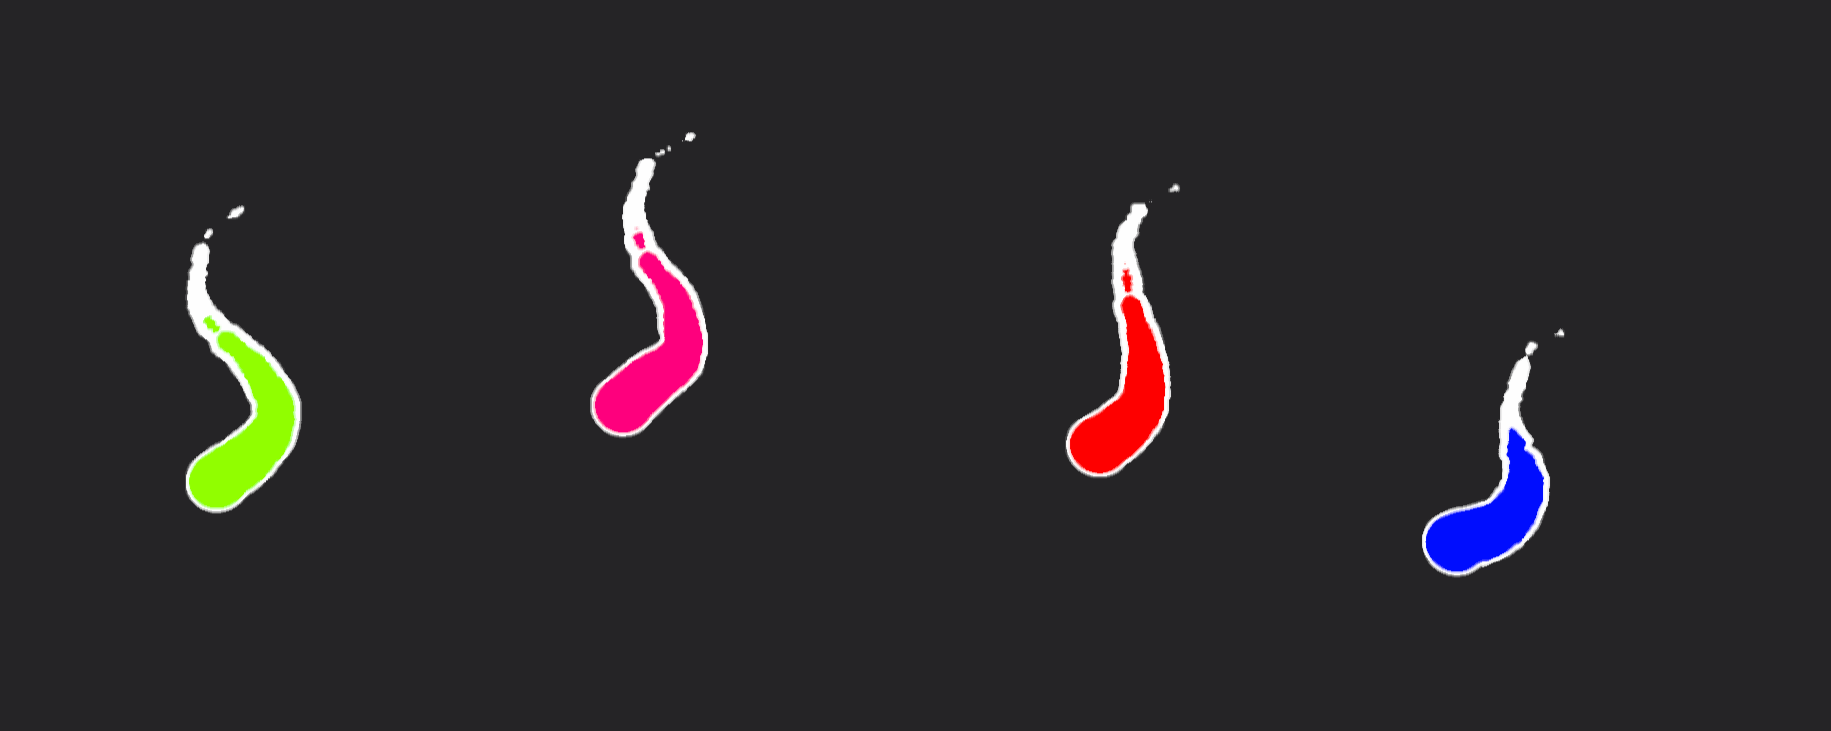
\includegraphics[width=1\textwidth]{figures/touch_indicators.png}
            \captionof{figure}{Touch indicators for four fingers on the touch frame.}
            \label{fig:touch_indicators}
        \end{figure}

        This is implemented using a compute shader and a shader built with Unity's Shader Graph. A compute shader is a program that runs on the GPU outside of the normal rendering pipeline.\footnote{\url{https://docs.unity3d.com/Manual/class-ComputeShader.html}} It is most useful for executing highly parallel algorithms. In this case, the compute shader processes finger positions, performs calculations, and stores results in render textures. The Shader Graph shader then uses these textures to render finger trail indicators in every frame.

        Each render texture stores data for two fingers using two channels per finger per pixel. This results in five textures, each with dimensions matching the greatest nearest power of two between the screen width and height. One channel stores the reverse distance from the pixel to the center of the finger trail, ranging from 1 (closest to the center) to 0 (outside the trail radius), similar to a signed distance function. The other channel records the decay of the pixel, where 1 indicates the most recent position, and 0 indicates total decay. These channels are depicted in Figure \ref{fig:touch_progress}, with red representing the distance to the trail's center and blue representing the decay.
        
        \begin{figure}[h!]
            \centering
            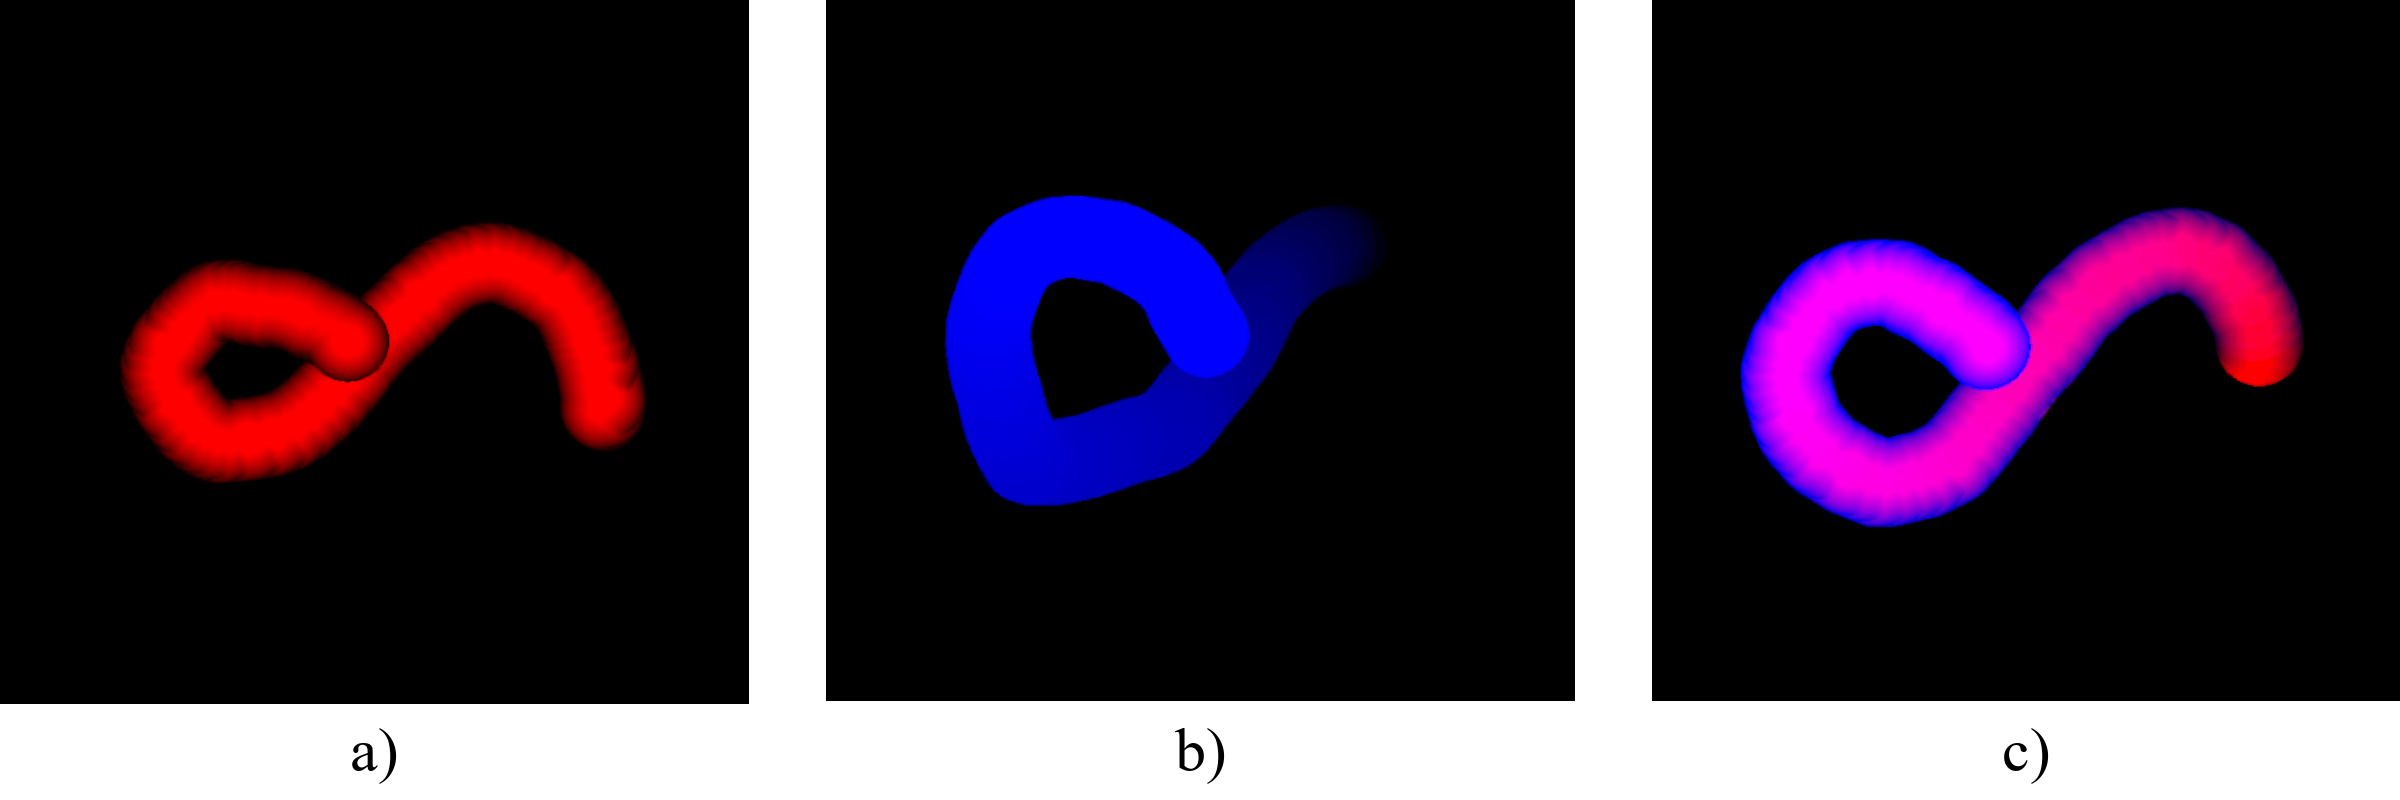
\includegraphics[width=1\textwidth]{figures/touch_progress.png}
            \captionof{figure}{The different components stored on the render texture for each finger: a) reverse distance to center; b) decay; c) distance and decay combined.}
            \label{fig:touch_progress}
        \end{figure}

        A compute shader function is executed by several compute shader thread groups for each of the three dimensions: \(X\), \(Y\), and \(Z\). In this case, the function defines for each group 8 threads for the \(X\) dimension, representing the pixel coordinate on the X axis, 8 threads for the \(Y\) dimension, representing the pixel coordinate on the Y axis, and 1 thread for the \(Z\) dimension, representing the render texture being processed. When the compute shader is executed, it runs using \(\text{texture}_{\text{width}} / 8\) groups on the \(X\) axis, \(\text{texture}_{\text{height}} / 8\) groups on the \(Y\) axis, and 5 groups on the \(Z\) axis, one for each render texture.

        The compute shader takes several inputs: five different render textures, two \lstinline{float4} structured buffers of size 5 (one for the current finger positions and one for the finger positions of the previous frame), a \lstinline{float} structured buffer of size 10 that stores the average inclination of each finger trail, a linear decay rate $\delta$, a finger radius in pixels $r$, and the time elapsed between the last frame and the current frame in seconds $\Delta t$. Each \lstinline{float4} vector in the structured buffers represents the screen-space coordinates of two fingers, with the first two floats for one finger and the next two floats for another finger.

        A simplified description of the algorithm for each finger and each pixel operates as follows: first, it calculates the decay \(\lambda_i\) of the pixel using the previous frame's decay value \(\lambda_{i-1}\) by computing \(\lambda_{i-1} - \delta \cdot \Delta t\). Next, it calculates the distance \(d\) and reverse distance $d_{\mathrm{rev}}$ from the pixel to the line segment that starts at the finger's position in the previous frame and ends at the current finger position. This calculation, shown in Equation \ref{eq:distance_line}, creates a capsule-like shape. In this equation, \(A\) is the finger's position in the last frame, \(B\) is the current finger's position, \(r\) is the line's thickness, and \(P\) is the pixel's position.

        \begin{figure}[h]
        \begin{equation}
        \begin{split} \label{eq:distance_line}
            \vec{AB} &= B - A \\
            \vec{AP} &= P - A \\
            h &= \mathrm{clamp} \left( \frac{\vec{AP} \cdot \vec{AB}}{\vec{AB} \cdot \vec{AB}} , 0, 1\right)  \\
            d &= \frac{\| \vec{AP} - h \cdot \vec{AB} \|}{r} \\
            d_{\mathrm{rev}} &= \mathrm{clamp} \left( 1 - d , 0 , 1\right)
        \end{split}
        \end{equation}
        \end{figure}

        %Then, it calculates how much the pixel is in front of the line segment using the calculating $h$ described in Equation \ref{eq:distance_line}, where $B$ is instead $(A_x + r \cdot \cos{\bar{m}}, A_y + r \cdot \sin{\bar{m}})$, where $\bar{m}$ is the average incline of the finger trail. The average incline is used instead of $B$ because often the line segments between frames are very small and one directional due to high refresh rates, resulting in visual artifacts.

        %Next, it checks whether the previously stored distance is still valid by checking whether $\lambda_i$ is less than $$~


        Based on how much the pixel is in front of the line segment, considering the average inclination of the finger trail, the algorithm linearly interpolates between \(\max\left(d_{\text{rev}}, d_{\text{rev}_{i-1}}\right)\) and \(d_{\text{rev}}\) to calculate the value to store in the render texture. This approach allows the finger trail to overlap at the front and smoothly blend behind. The final decay value stored in the texture is \(\lambda_i\), with an additional 1 added if \(d \leq 1\), clamped between 0 and 1.

        Finally, the fragment shader samples each render texture. It subtracts the decay value from the distance to create a shrinking effect, applies a border by comparing the resulting value with a threshold, and assigns a color based on the finger's order.

        \begin{figure}[h!]
            \centering
            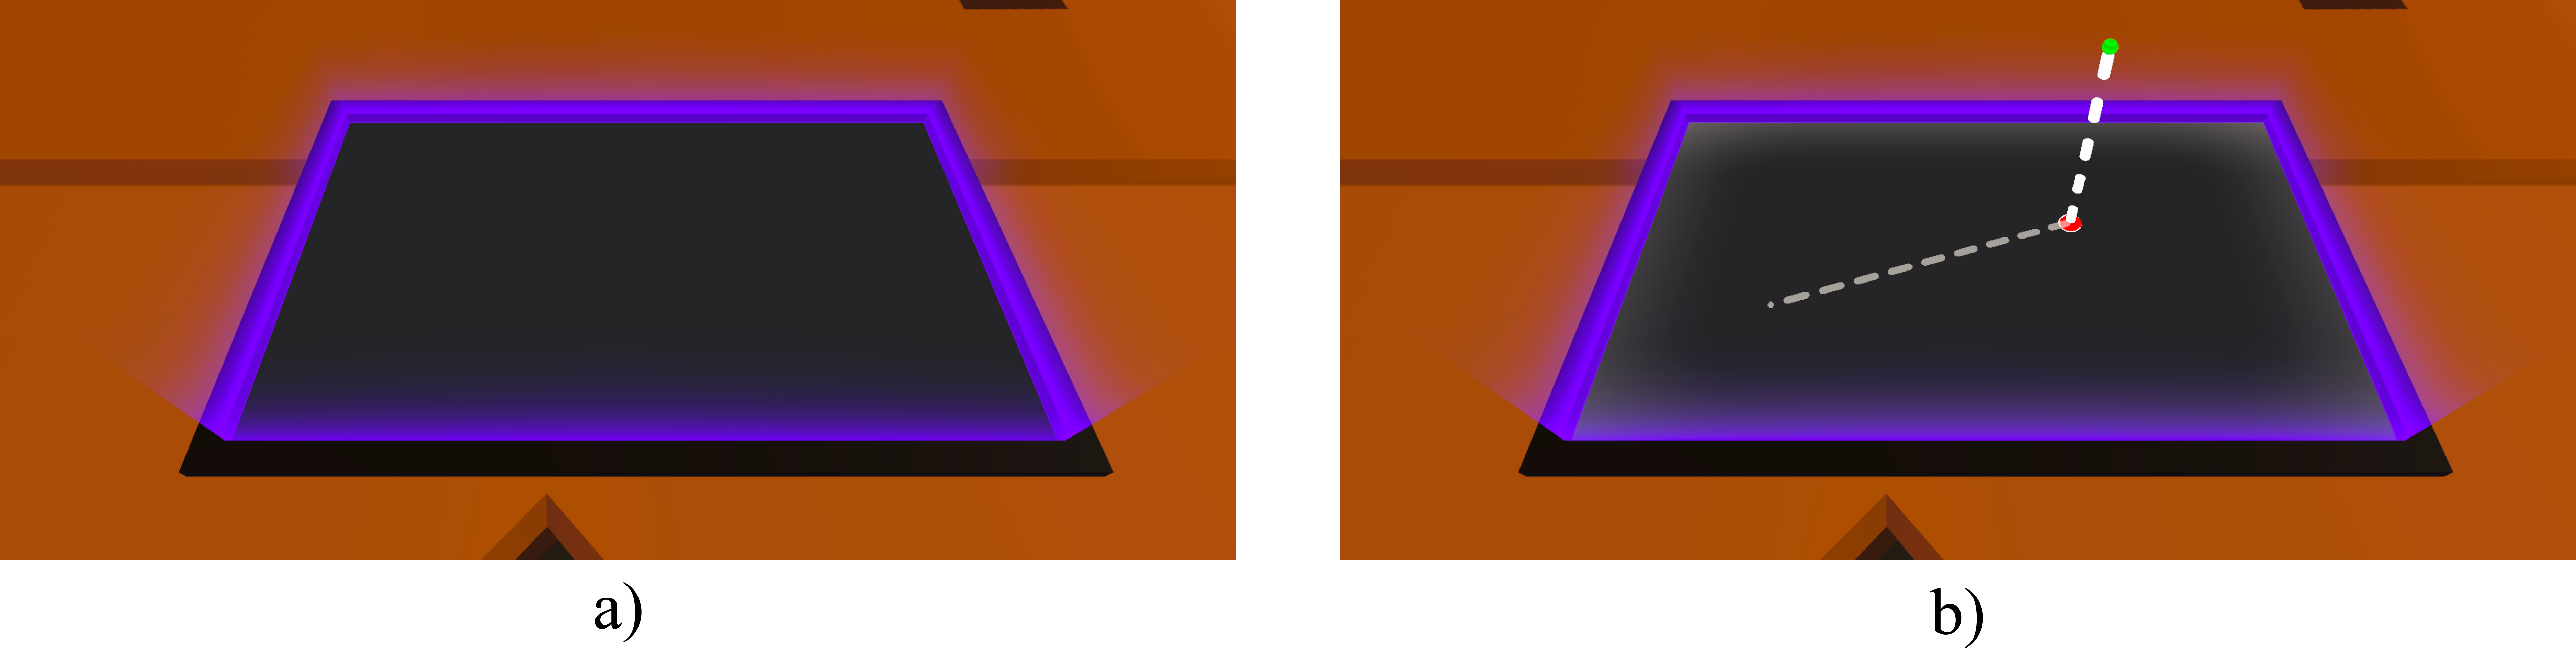
\includegraphics[width=1\textwidth]{figures/frame_glow.png}
            \captionof{figure}{Glow effect indicating gesture detection on the touch surface. (a) The initial state with no gesture detected. (b) The glow effect activates when a gesture is detected.}
            \label{fig:frame_glow}
        \end{figure}

        The virtual touch frame illuminates with a glowing effect whenever the system detects vertical transform or balloon selection gestures, signaling the user that their gesture has been recognized. This glow effect, demonstrated in Figure \ref{fig:frame_glow}, is achieved using a shader that uses a rounded box signed distance function.\footnote{\url{https://www.shadertoy.com/view/Nlc3zf}} The strength of the glow is animated using the function $-\left(2 \sqrt{t} - 1\right)^2 + 1$, where \(t\) represents the elapsed time since the animation began. Initially, this function rises quickly until the result reaches 1 at $t = 0.25$, after which it gradually diminishes. The animation halts at \(t = 0.8\) and resumes from that point when the gesture concludes.
                    


        %\begin{figure}[h!]
        %    \centering
        %    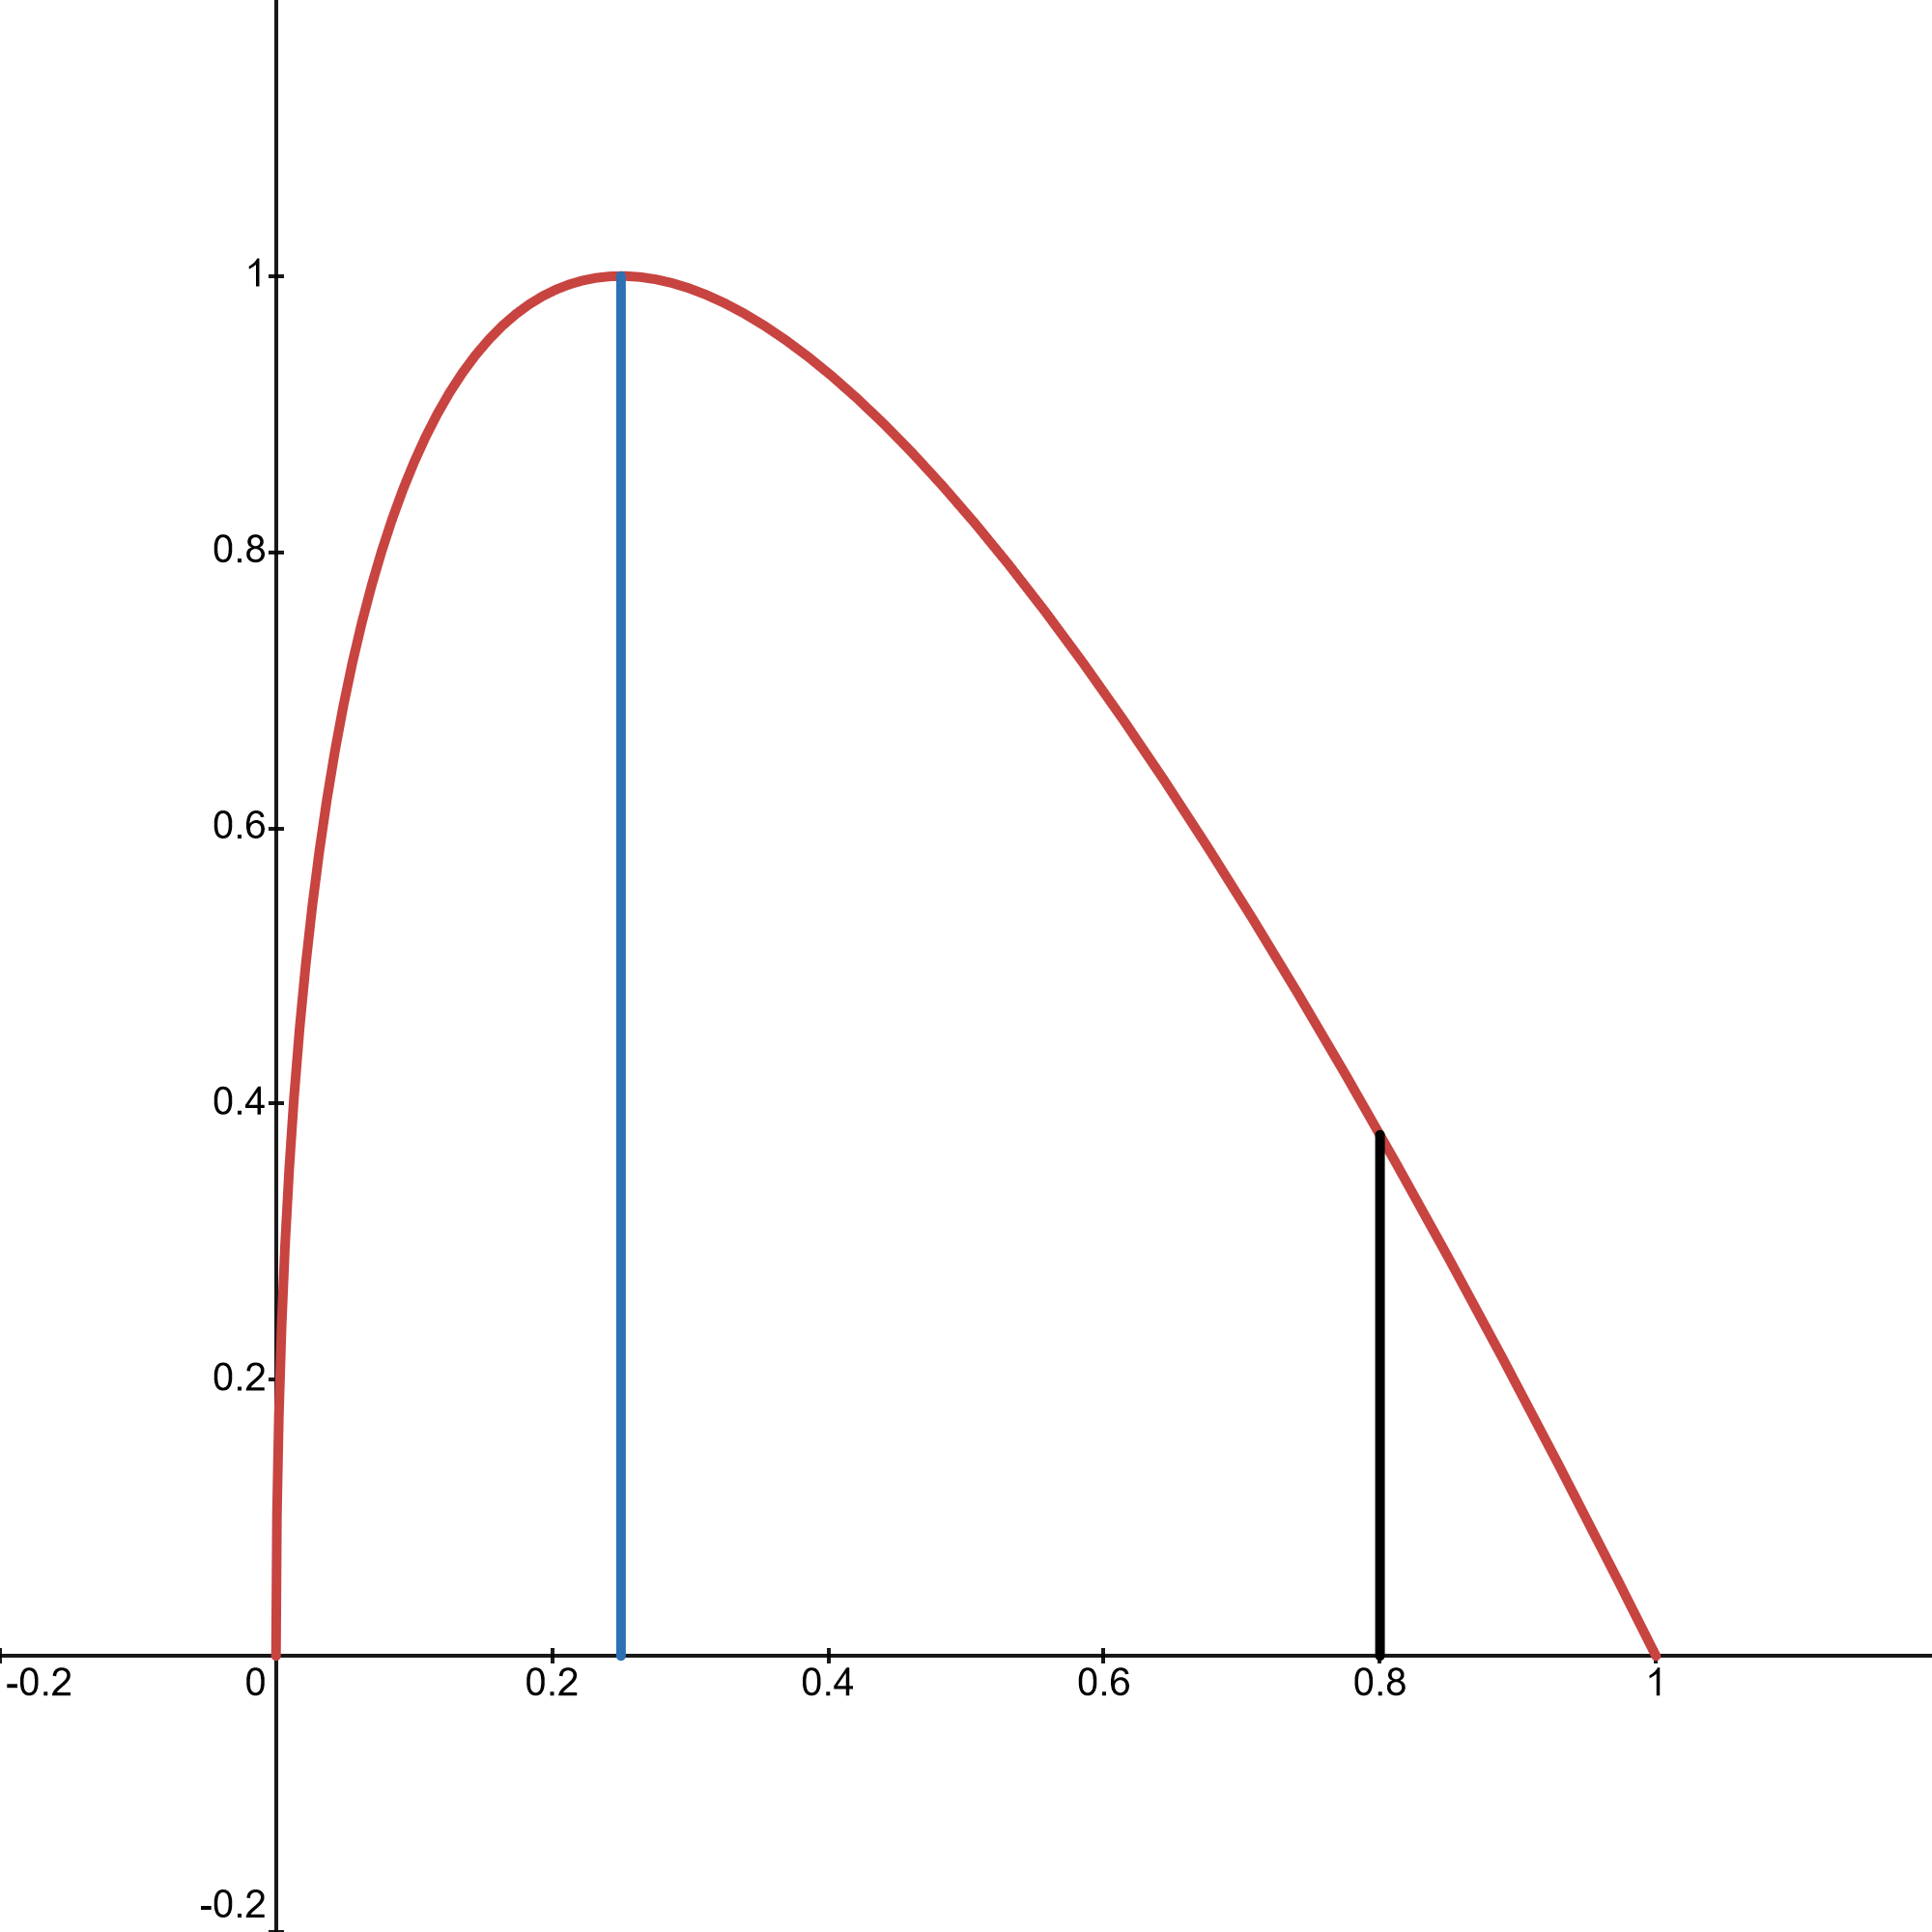
\includegraphics[width=0.5\textwidth]{figures/frame_glow_f.png}
        %    \captionof{figure}{Animation curve for the strength of the glow effect. The blue line at \( t = 0.25 \) indicates the point of maximum strength, and the line at \( t = 0.8 \) marks where the animation halts.}
        %    \label{fig:frame_glow}
        %\end{figure}
    
    
    \subsection{Frame Limit Indicator} \label{sec:frame_limits}

        The balloon's position on the XZ axis during balloon selection is constrained by the boundaries of the virtual touch frame. To help users understand these boundaries, even when the frame is obscured by the replica, a purple illumination effect outlines the limits. This effect is shown in Figure \ref{fig:frame_limits}.

        \begin{figure}[h!]
            \centering
            \includegraphics[width=1\textwidth]{figures/frame_limits.png}
            \captionof{figure}{Illumination effect on the replica indicating the limits of the touch frame.}
            \label{fig:frame_limits}
        \end{figure}
    
        The illumination effect is achieved using a shader applied to a transparent rectangular prism extending from the touch frame's base. The shader's primary function is to gradually diminish the illumination effect as the distance from the prism increases. This is accomplished using a modified version of a shader initially designed for a stylized water effect\footnote{\url{https://ameye.dev/notes/stylized-water-shader/}}, created using Unity's Shader Graph.
        
        To calculate the distance \( d \), a vector \(\vec{CA}\) is obtained from the camera to the fragment's position on the prism using the View Vector node. This vector is then normalized to \(\hat{v}\). The depth texture is sampled to obtain the distance from the camera to the point occluded by the prism, \(|CB|\). The normalized vector is multiplied by this distance, resulting in \(\vec{CB} = \hat{v} \cdot |CB|\). Adding this vector to the camera's position gives the position of the occluded point, \( B = C + \vec{CB} \). The distance vector \(\vec{BA}\) is obtained by subtracting the occluded point's position from the fragment's position on the prism's surface, \(\vec{BA} = A - B\). Finally, the length of this vector is calculated to obtain the distance, \( d = \|\vec{BA}\| \).
        
        \begin{figure}[h!]
            \centering
            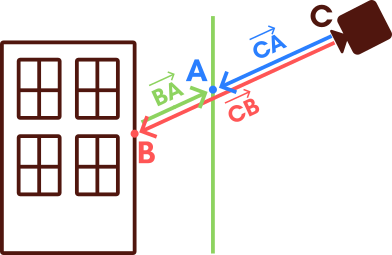
\includegraphics[width=.5\textwidth]{figures/limit_calc.png}
            \captionof{figure}{Diagram illustrating the steps to calculate $d$.}
            \label{fig:limit_calc}
        \end{figure}
    
        To achieve the gradual effect, the function \( x = e^{-\frac{d}{0.05}} \) is applied. This ensures that when \( d = 0 \), the effect is at full power, declines rapidly, and then tapers off. This behavior is shown in graph a) of Figure \ref{fig:limit_func}. To soften the effect at the borders, the function described in Equation \ref{eq:limit_calc} and depicted in graph b) of Figure \ref{fig:limit_func} is applied to \( x \). This adjustment causes the effect to start at 0.2 power at the border, rise smoothly to 0.8 power, and then taper off as the distance increases. This progression is illustrated in graph c) of Figure \ref{fig:limit_func}.

        The function \( -37.5 x^3 + 82.5 x^2 - 60 x + 15.2 \) was derived from a cubic polynomial for creating a smooth curve between two points: \((c, m)\) and \((k, m + b)\), shown in Equation \ref{eq:limit_poly}.\footnote{\url{https://math.stackexchange.com/a/2209953}} In this case, the parameters are \( c = 0.8 \), \( m = 0.8 \), \( k = 1 \), \( b = -0.6 \), \( p = 0 \), and \( q = -1.5 \).

        \begin{figure}[h]
        \begin{equation} \label{eq:limit_calc}
        \alpha =
        \begin{cases}
            x & \text{if} \quad x \leq 0.8 \\
            -37.5 x^3 + 82.5 x^2 - 60 x + 15.2 & \text{if} \quad x > 0.8 \\
            0.2 & \text{if} \quad x > 1
        \end{cases}
        \end{equation}
        \end{figure}

      \begin{figure}[h]
        \begin{equation} \label{eq:limit_poly}
        \left(p+q-2\cdot b\right)\cdot\left(\frac{x-c}{k-c}\right)^{3}\ +\ \left(3\cdot b\ -\ 2\cdot p-q\right)\cdot\left(\frac{x-c}{k-c}\right)^{2\ }+\ p\ \cdot\ \left(\frac{x-c}{k-c}\right)+m
        \end{equation}
        \end{figure}

                
        \begin{figure}[h!]
            \centering
            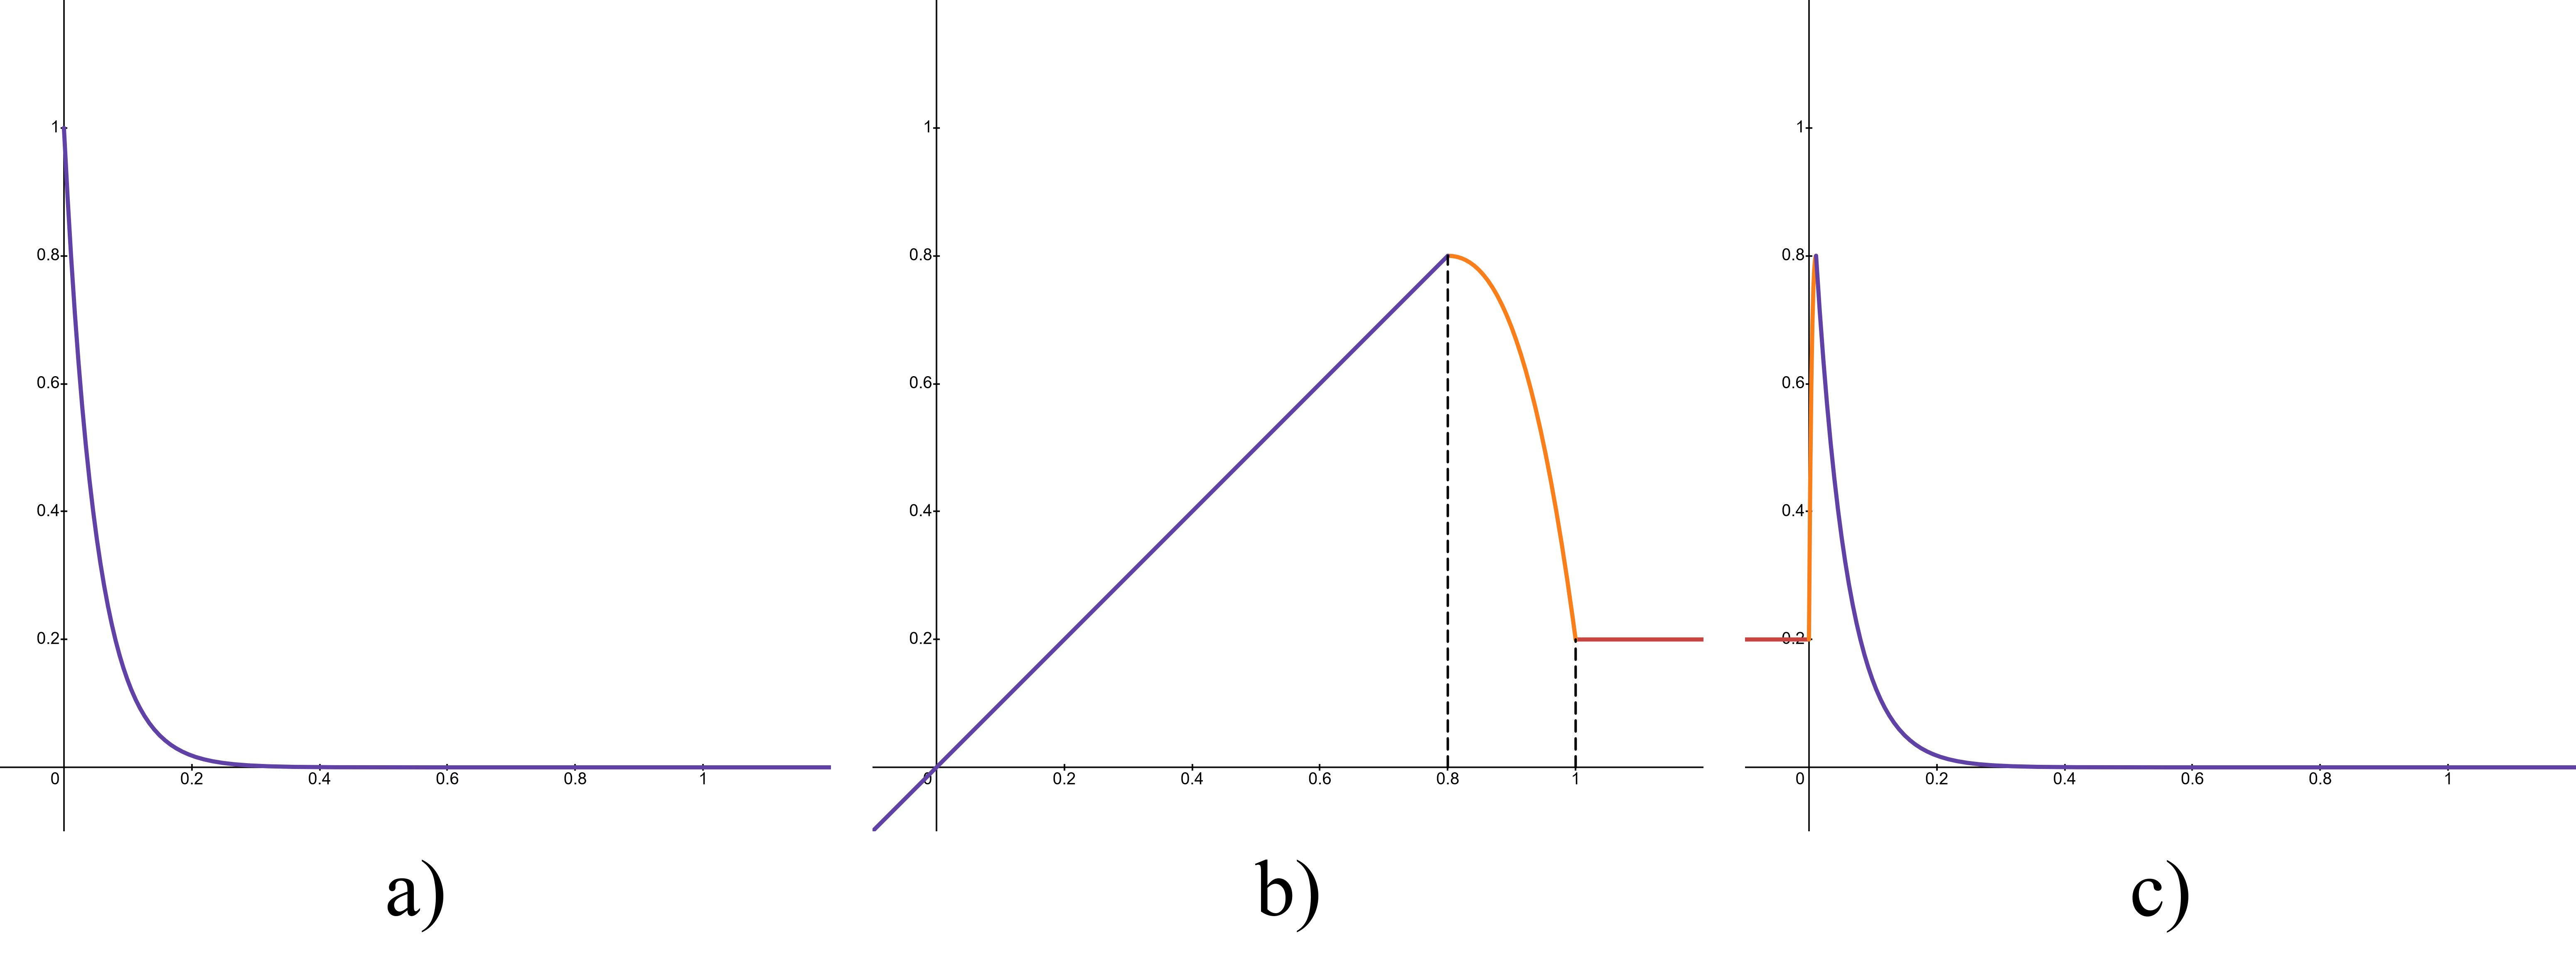
\includegraphics[width=1\textwidth]{figures/limit_func.png}
            \captionof{figure}{Graphs illustrating the functions used to modify the intensity of the limit illumination effect. Graph a) shows \( e^{-\frac{d}{0.05}} \) where the horizontal axis represents distance \( d \). Graph b) displays the function described in Equation \ref{eq:limit_calc}, with the horizontal axis representing \( x \). Graph c) depicts the function from Equation \ref{eq:limit_calc} with the horizontal axis representing distance \( d \). }
            \label{fig:limit_func}
        \end{figure}

    \subsection{Virtual Table} \label{sec:virtual_table}

        As shown in the literature \cite{zielaskoMenusDeskSystem2019, sousaVRRRRoomVirtualReality2017, zielaskoNonStationaryOfficeDesk2019}, the presence of a virtual table can be helpful in presenting information. This prototype uses the virtual touch frame described in Section \ref{sec:touch_frame} to represent that information. While the table is useful for displaying information, it can obscure much of the to-scale model, especially if the user wants to look down. To make it less intrusive, the table begins to fade and becomes invisible after 2 seconds of the touch surface not detecting any fingers, as shown in Figure \ref{fig:table_visibility}.

        \begin{figure}[h!]
            \centering
            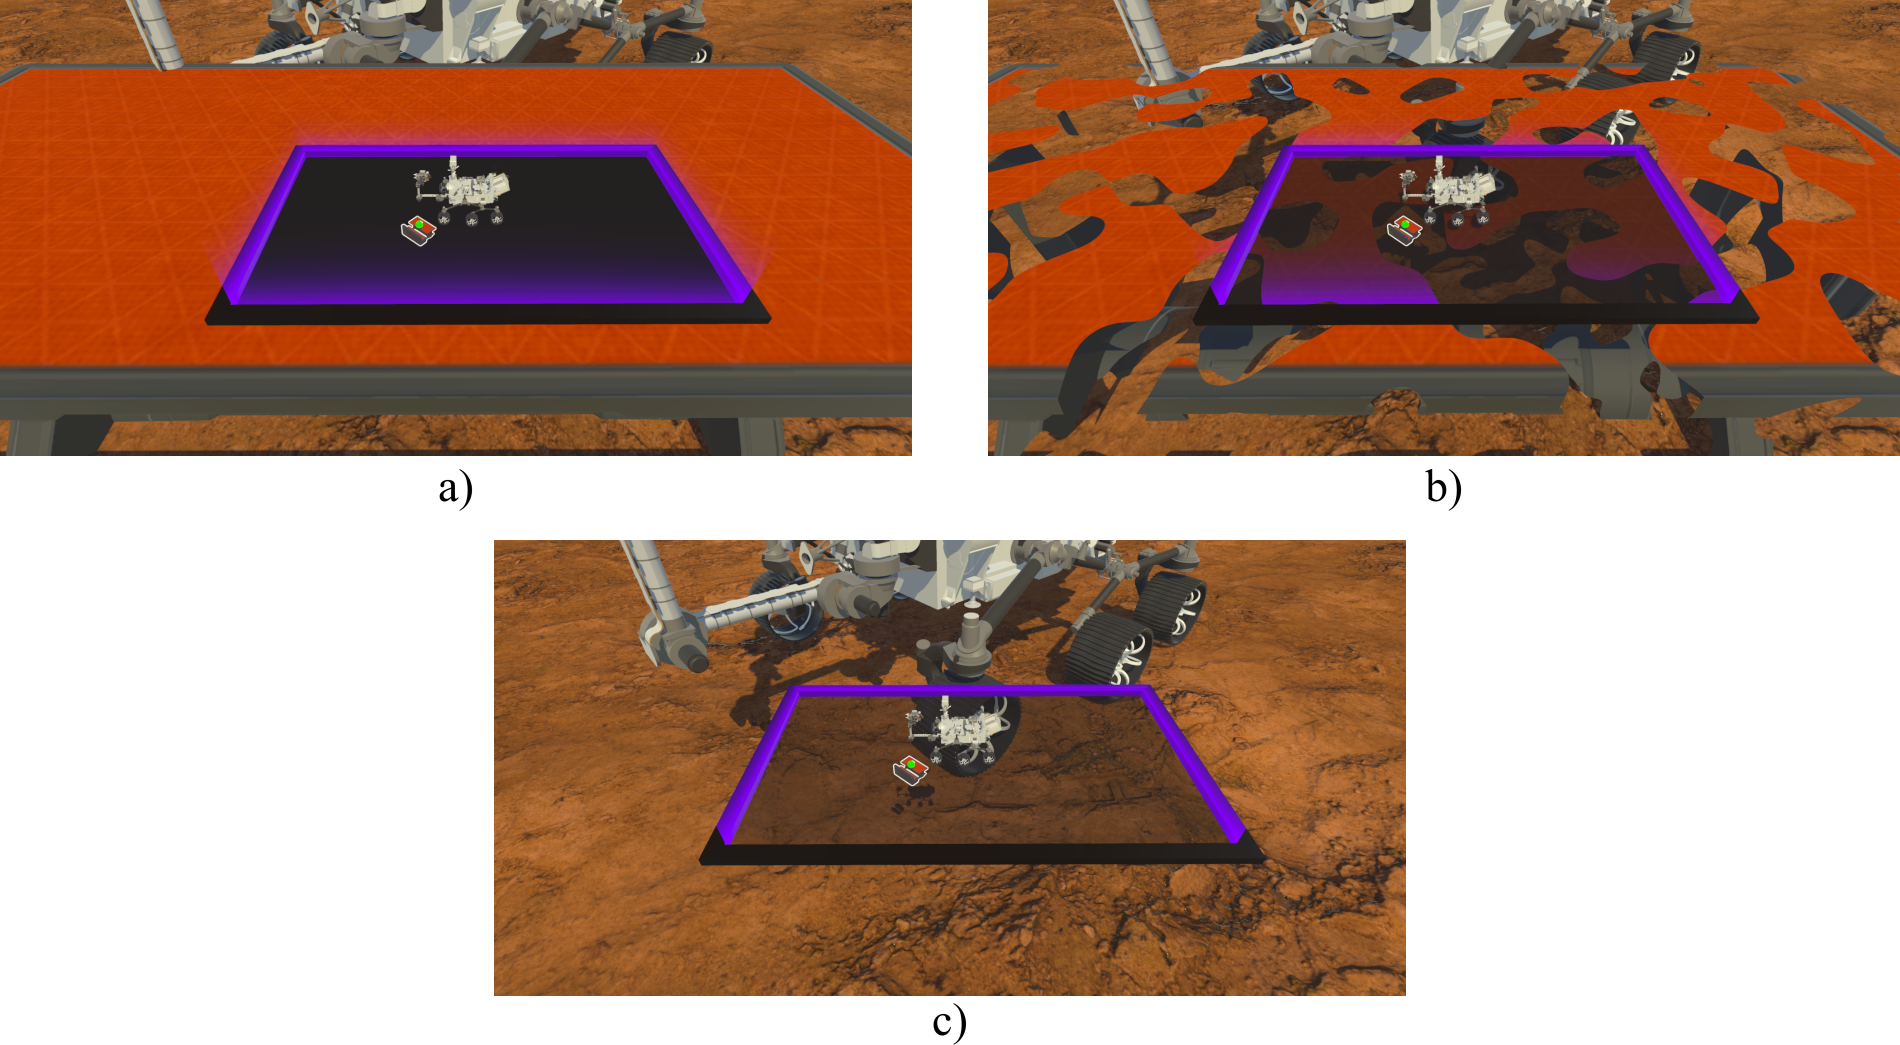
\includegraphics[width=1\textwidth]{figures/table_visibility.png}
            \captionof{figure}{The transition of the virtual table from: a) fully visible; b) half-visible; c) fully invisible.}
            \label{fig:table_visibility}
        \end{figure}

        This effect is achieved using a shader that takes the pixel's world space position and applies a simplex 3D noise function\footnote{\url{https://github.com/JimmyCushnie/Noisy-Nodes}} to determine the pixel's alpha clip threshold. After 2 seconds of inactivity, the table's alpha value is reduced using a smooth animation curve. The alpha clip threshold then determines whether a pixel is visible or invisible. Alpha blending was not used because it caused visual artifacts, making the table visible from behind itself.

        User tables are also visible in the replica as miniatures, as shown in Figure \ref{fig:table_behind} and described in Section \ref{sec:awareness}. These miniatures feature an outline effect to help them stand out from the surrounding environment, using a free Unity package.\footnote{\url{https://assetstore.unity.com/packages/tools/particles-effects/quick-outline-115488}} They also glow intermittently to draw attention, increasing the lightness of the table's color through an animation using a quadratic easing in-out function.\footnote{\url{https://assetstore.unity.com/packages/vfx/shaders/shader-graph-easing-193427}} The miniatures display who is at the table by showing a user seated at it, as seen in image c) of Figure \ref{fig:table_behind}. These miniatures do not scale with the replica, keeping their size constant, similar to markers on a map. They remain visible behind objects in the replica to help users quickly identify their and others' tables. This is achieved by rendering the table miniature in an additional render pass using the depth buffer to determine the appropriate material. If the table is behind an object, it appears slightly transparent and in a single color; otherwise, it uses the normal material.\footnote{\url{https://docs.unity3d.com/Packages/com.unity.render-pipelines.universal@10.4/manual/renderer-features/how-to-custom-effect-render-objects.html}}

        \begin{figure}[h!]
            \centering
            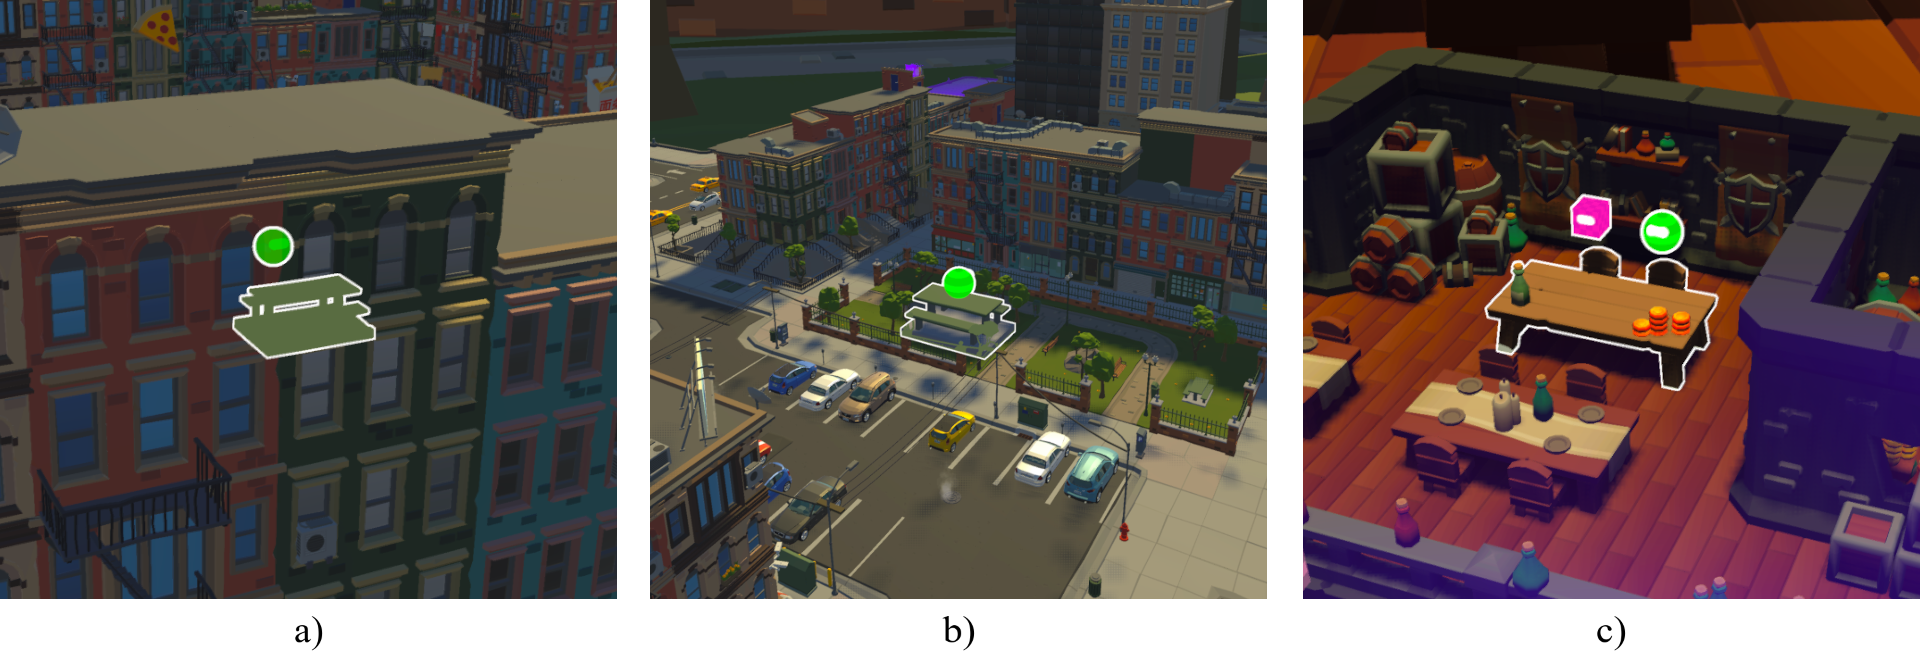
\includegraphics[width=1\textwidth]{figures/table_behind.png}
            \captionof{figure}{The table miniature visible in the replica. Image (a) shows the table behind an object, image (b) shows the table within the replica, and image (c) shows two users at the table.}
            \label{fig:table_behind}
        \end{figure}


    \subsection{Points of Interest} \label{sec:visual_poi}
        As mentioned in Section \ref{sec:awareness}, the points of interest reflect the appearance of their creators. Figure \ref{fig:poi_appearance} demonstrates this: the first user's points of interest are green-striped spheres, while the second user's are purple checkerboard cubes. Each point of interest is marked with a number that rotates to face the camera and glows intermittently to draw attention, achieved using a Fresnel effect with a sine curve animation.

        \begin{figure}[h!]
            \centering
            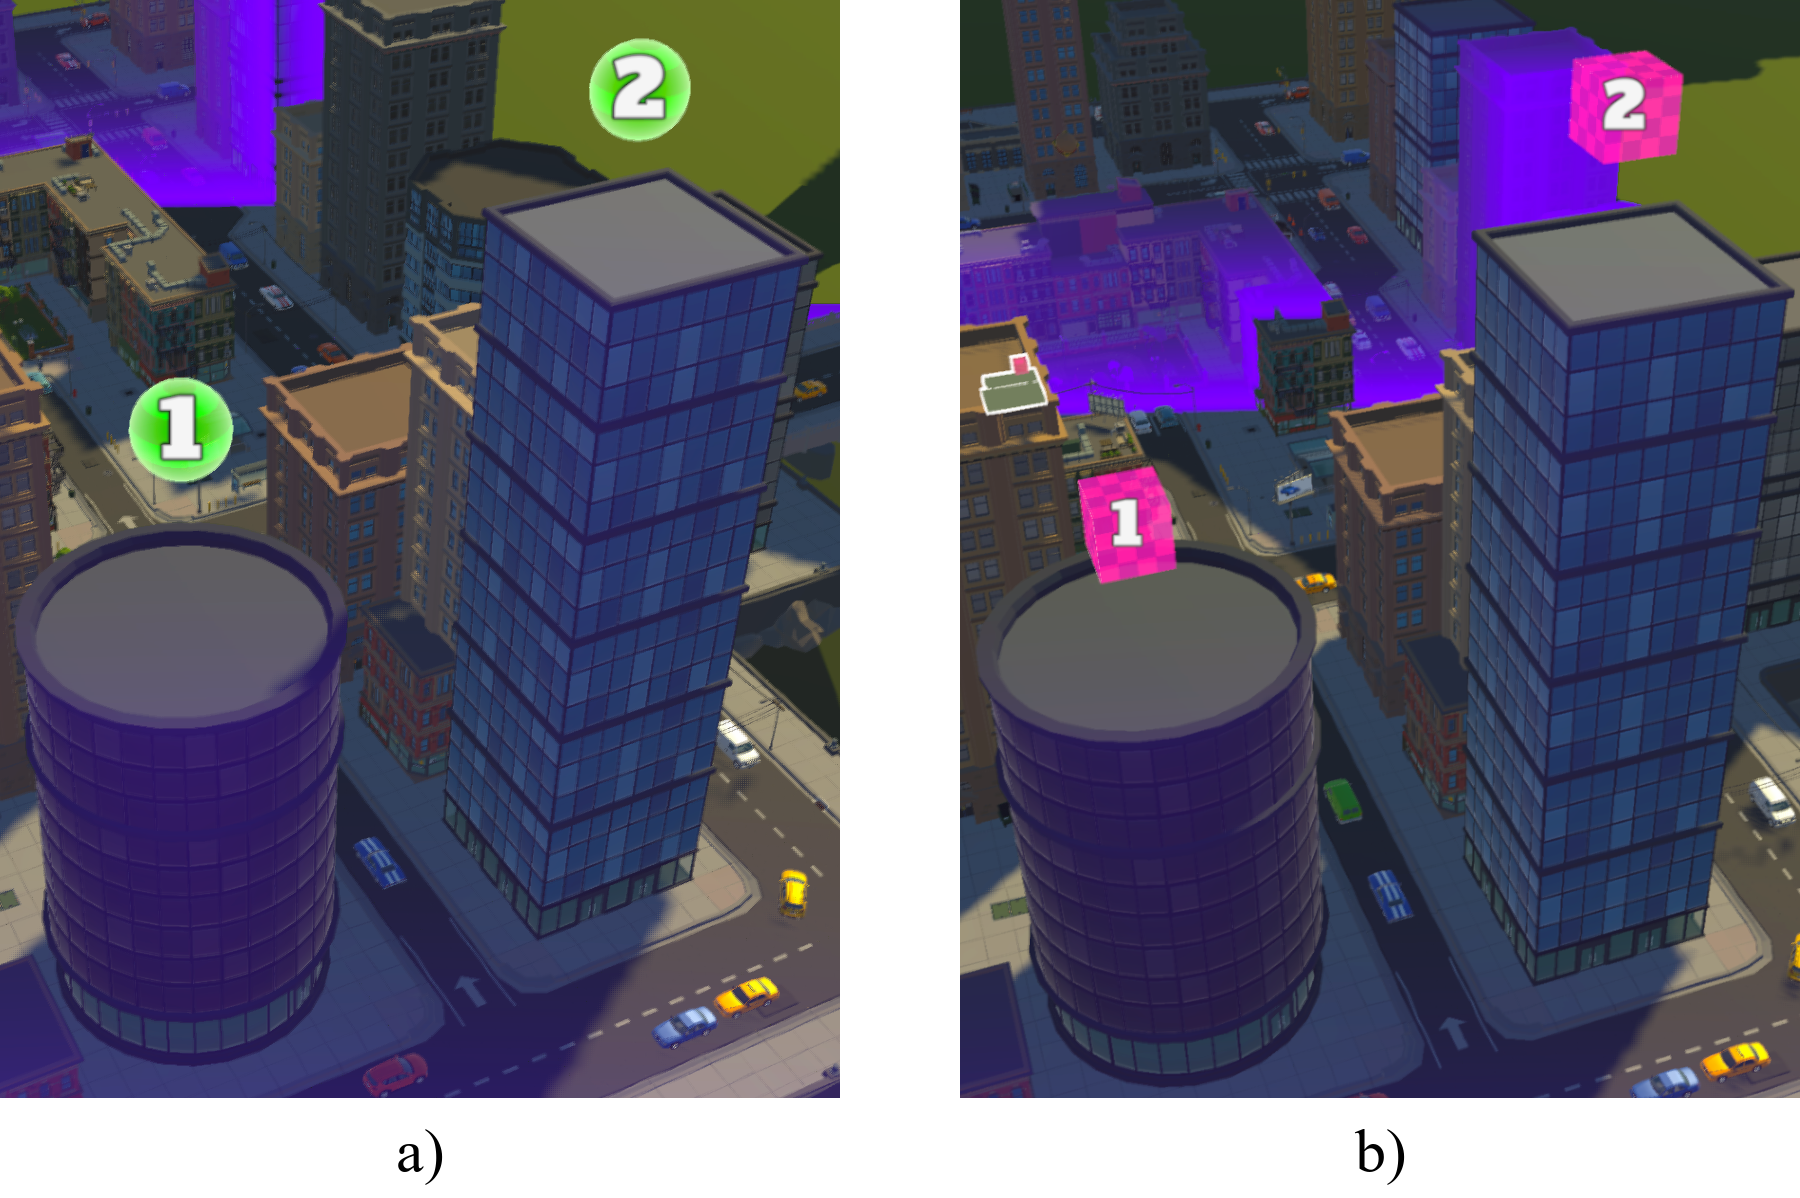
\includegraphics[width=.8\textwidth]{figures/poi_appearance.png}
            \captionof{figure}{Point of interest appearance based on the creator's appearance. Image (a) shows points of interest from the first user, and image (b) shows points of interest from the second user.}
            \label{fig:poi_appearance}
        \end{figure}

        Similar to the miniature tables, points of interest are visible behind objects in the replica and do not scale with the replica. This is shown in image (a) of Figure \ref{fig:poi_visibility}, where a point of interest is visible behind a building in the replica with a muted color and slight transparency. However, in the 3D model, the point of interest is not visible behind the building, as shown in image (b). This ensures that the points of interest do not distract or confuse users when looking at the replica. Points of interest in the 3D model scale with distance so users can see them from afar but do not become too large when close, preserving essential details.

       \begin{figure}[h!]
            \centering
            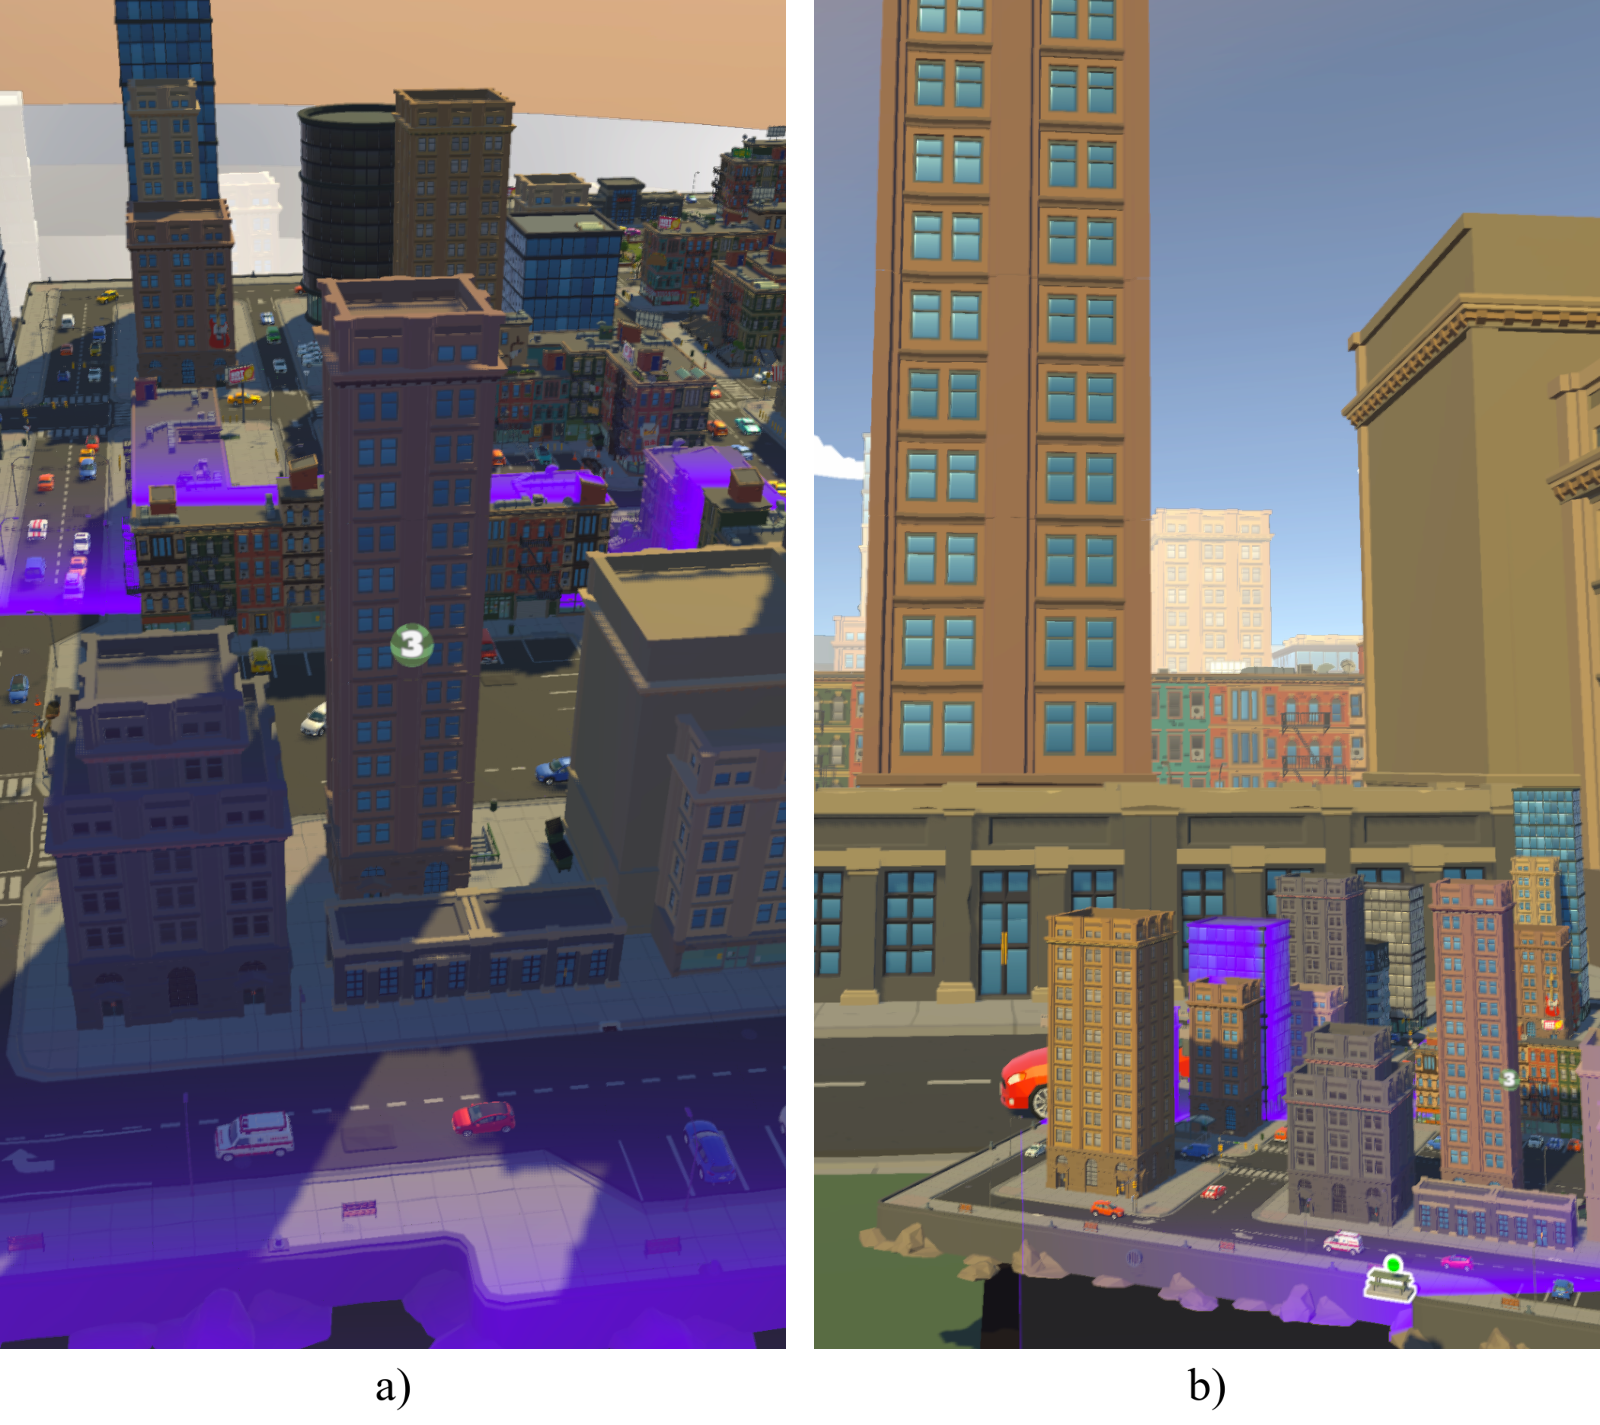
\includegraphics[width=.8\textwidth]{figures/poi_visibility.png}
            \captionof{figure}{Points of interest visibility. Image (a) shows a point of interest in the replica that is visible behind the building. Image (b) shows that the same point of interest is not visible in the 3D model behind the building.}
            \label{fig:poi_visibility}
        \end{figure}

        Points of interest created by another user that are not yet acknowledged are marked with a vertical line, as shown in Figure \ref{fig:poi_marker}. This line is capped with a symbol displaying the point of interest's identification number, resembling the point of interest's appearance to help users quickly identify unacknowledged points. The line and symbol always face the user using a vertical billboard effect. The line is also visible behind objects in the replica and scales with distance, as seen in image (c) of Figure \ref{fig:poi_marker}, ensuring it can be seen from any angle. If the marker does not fit within the user's field of view, it flips upside down to remain visible, as shown in image (d) of Figure \ref{fig:poi_marker}.

       \begin{figure}[h!]
            \centering
            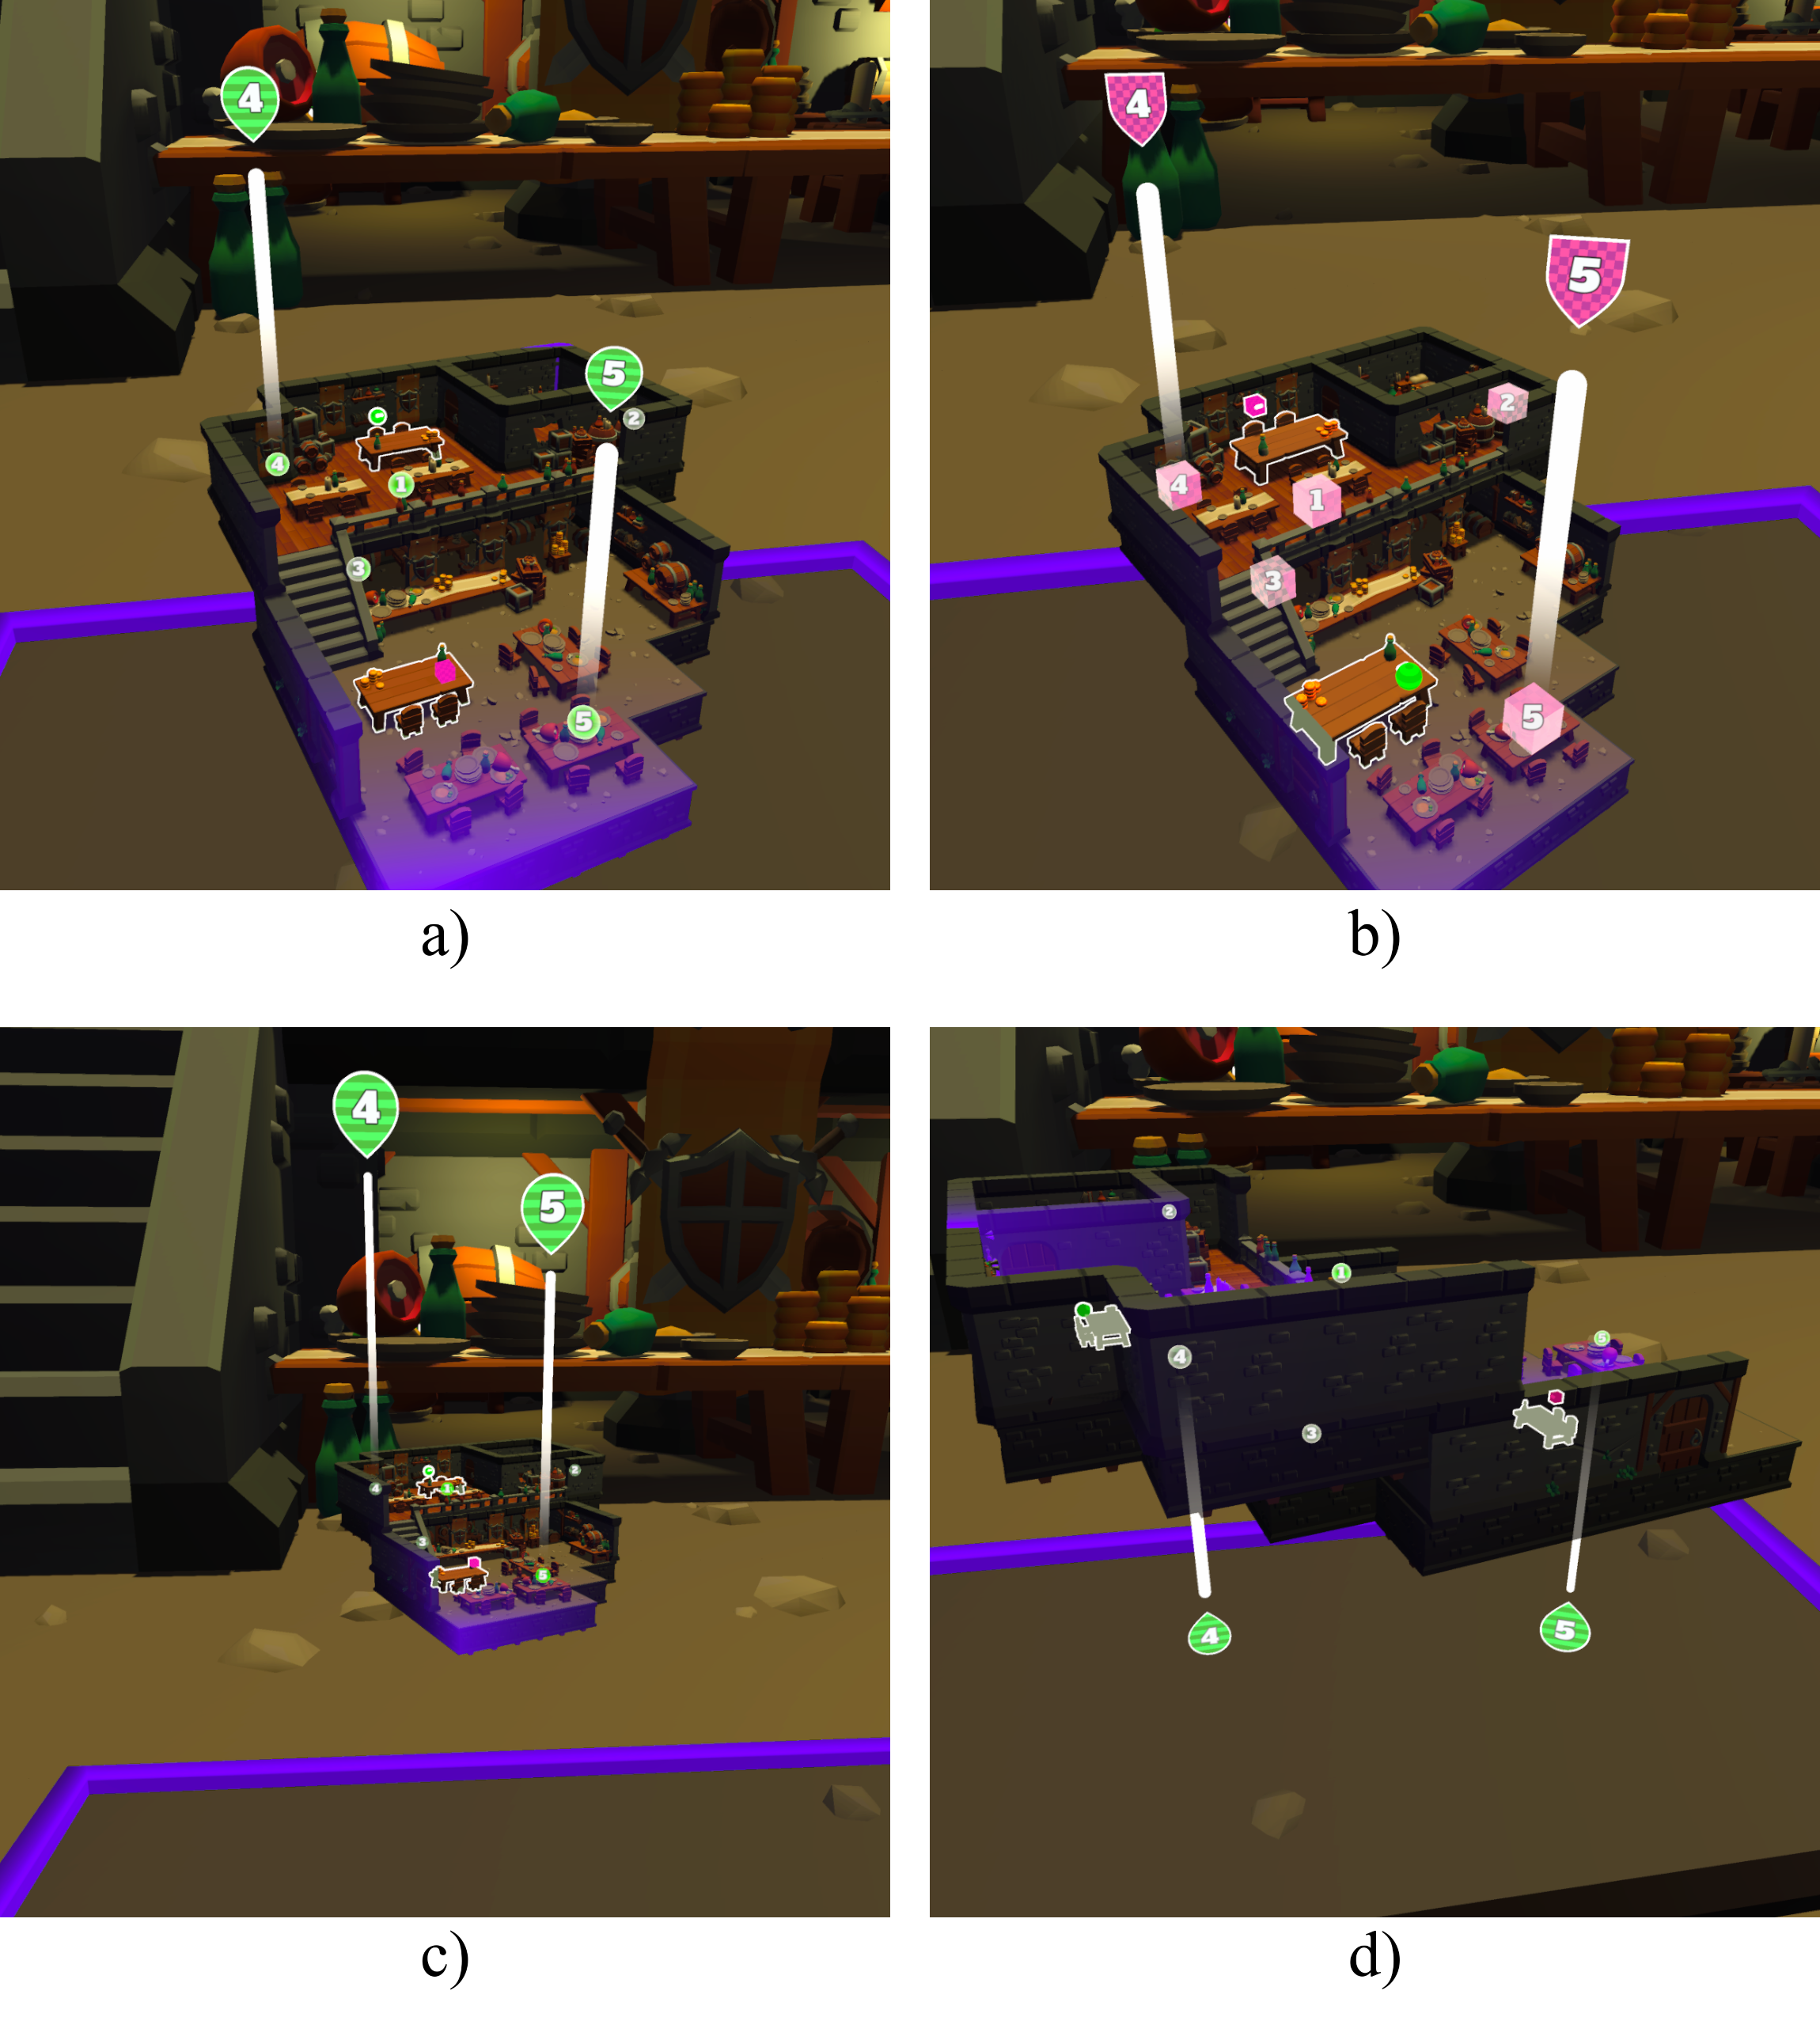
\includegraphics[width=1\textwidth, height=1\textheight, keepaspectratio]{figures/poi_marker.png}
            \captionof{figure}{Point of interest markers. Image (a) shows markers for the first user, and image (b) shows markers for the second user. Image (c) demonstrates the scaling of the markers with distance. Image (d) displays the markers flipped upside down to ensure they are always visible.}
            \label{fig:poi_marker}
        \end{figure}
        
    \subsection{Balloon Selection} \label{sec:visual_balloon}
        The balloon selection gesture is indicated by a set of dashed helper lines: one on the touch frame connecting the primary and secondary hands, and another vertical line from the primary hand to the balloon, using a vertical billboard effect, as shown in Figure \ref{fig:balloon_poi}. The balloon follows the appearance of the creator's points of interest. The helper lines and the balloon are visible behind objects in the replica with reduced opacity. When the secondary hand is inactive, the helper line on the touch frame loses its opacity, as shown in image (b) of Figure \ref{fig:balloon_poi}. If a segment of that line is behind an object and the secondary hand is inactive, that segment becomes invisible.

        The dashed lines are created using a shader that takes the positions of the hands, calculates the start and end positions of the dash segments using the percentages for each dash and gap, then draws the dash segments based on the calculations described in Equation \ref{eq:distance_line}. The dash segments at the ends are masked with a line from the start to the end position to ensure they have rounded ends.

        \begin{figure}[h!]
            \centering
            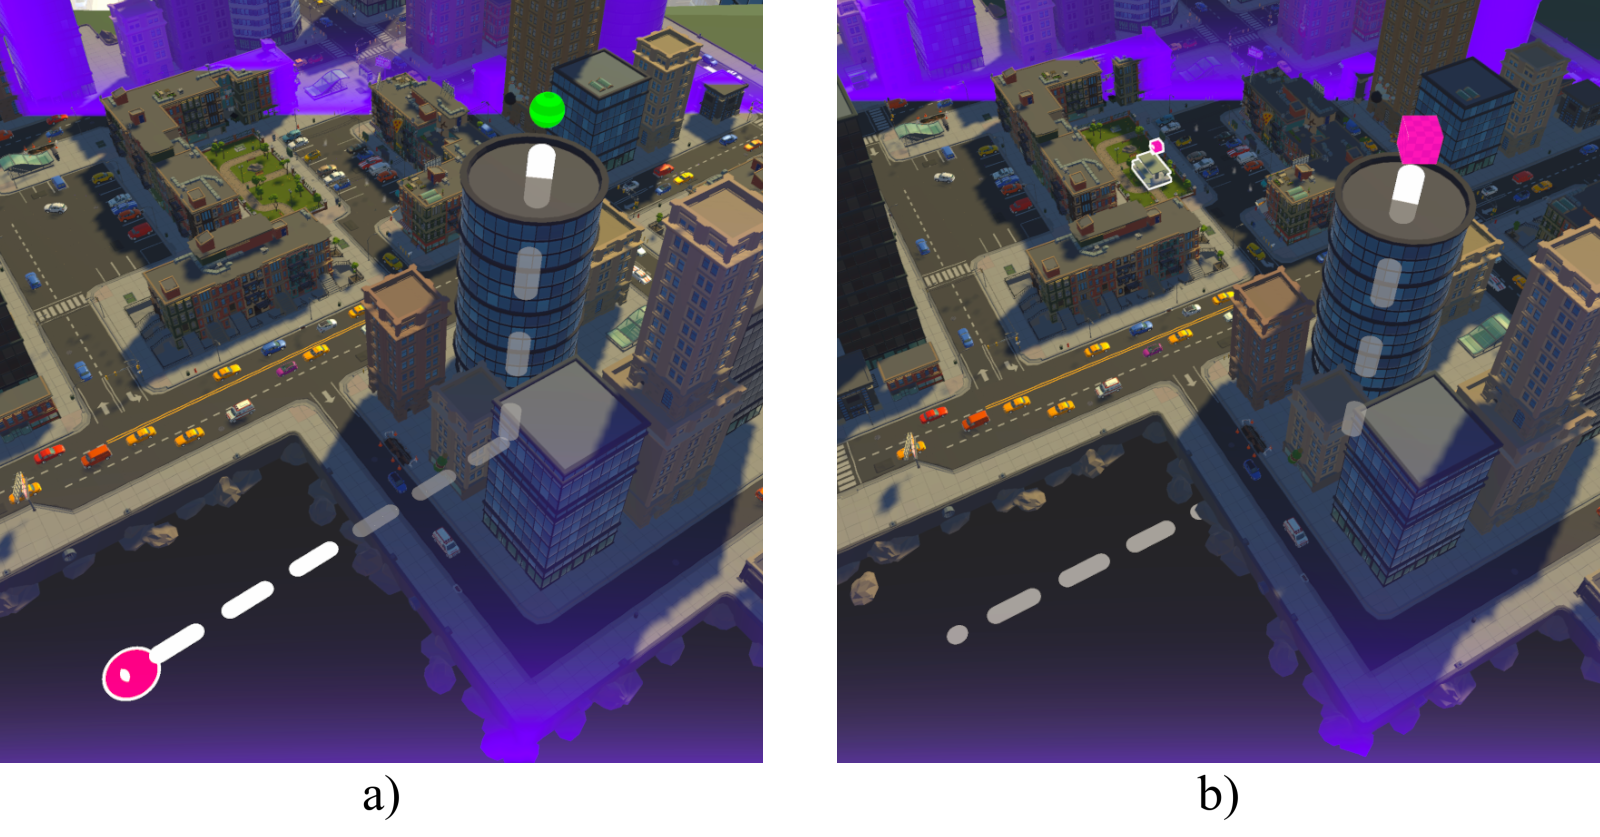
\includegraphics[width=1\textwidth]{figures/balloon_poi.png}
            \captionof{figure}{Balloon selection helper lines. Image (a) shows the balloon for the first user, and image (b) shows the balloon for the second user with the secondary hand removed.}
            \label{fig:balloon_poi}
        \end{figure}

        The balloon and the vertical helper line are also visible in the 3D model, as shown in Figure \ref{fig:balloon_world}, helping users understand the balloon's position in the real world. Both are not visible behind objects in the 3D model. The balloon scales with distance so users can see it from afar.

       \begin{figure}[h!]
            \centering
            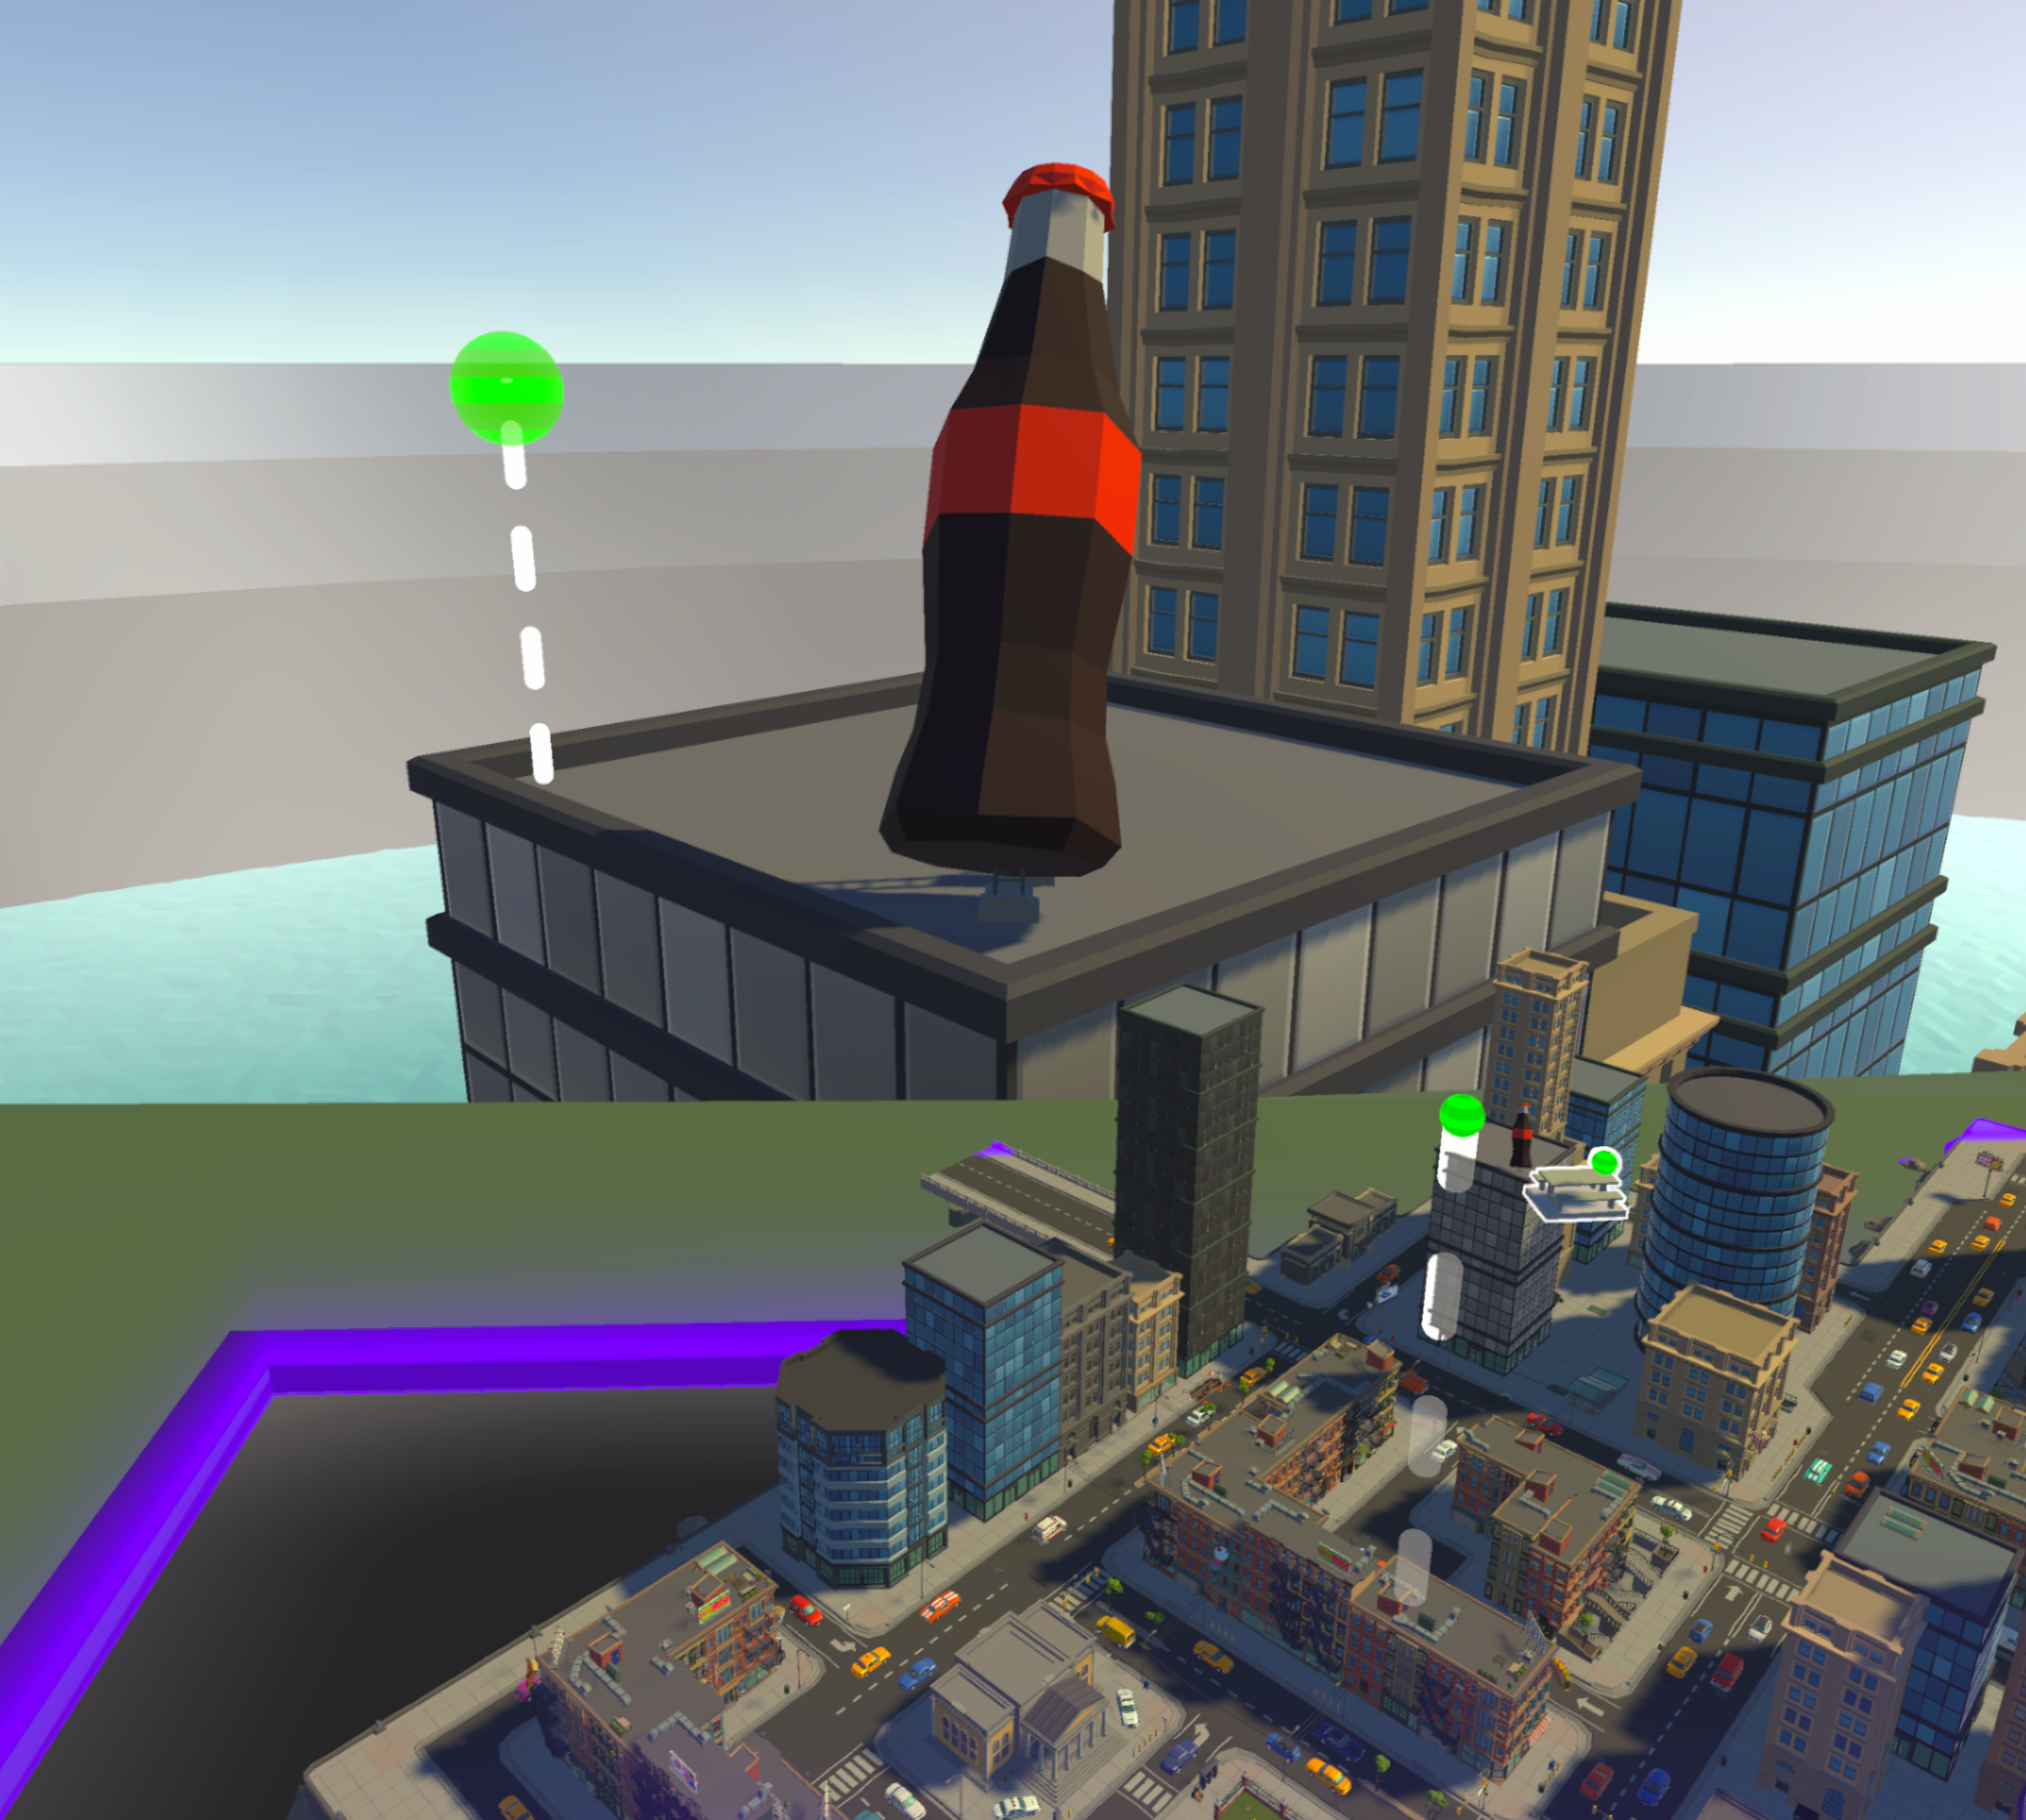
\includegraphics[width=1\textwidth]{figures/balloon_world.png}
            \captionof{figure}{Balloon selection visible both in the replica and in the 3D model.}
            \label{fig:balloon_world}
        \end{figure}
        
        When the balloon intersects a point of interest, the point of interest becomes outlined, indicating it is selected, as shown in image (a) of Figure \ref{fig:balloon_selection_intersection}. When the balloon intersects a table, the table grows in size, as shown in image (b) of Figure \ref{fig:balloon_selection_intersection}.

       \begin{figure}[h!]
            \centering
            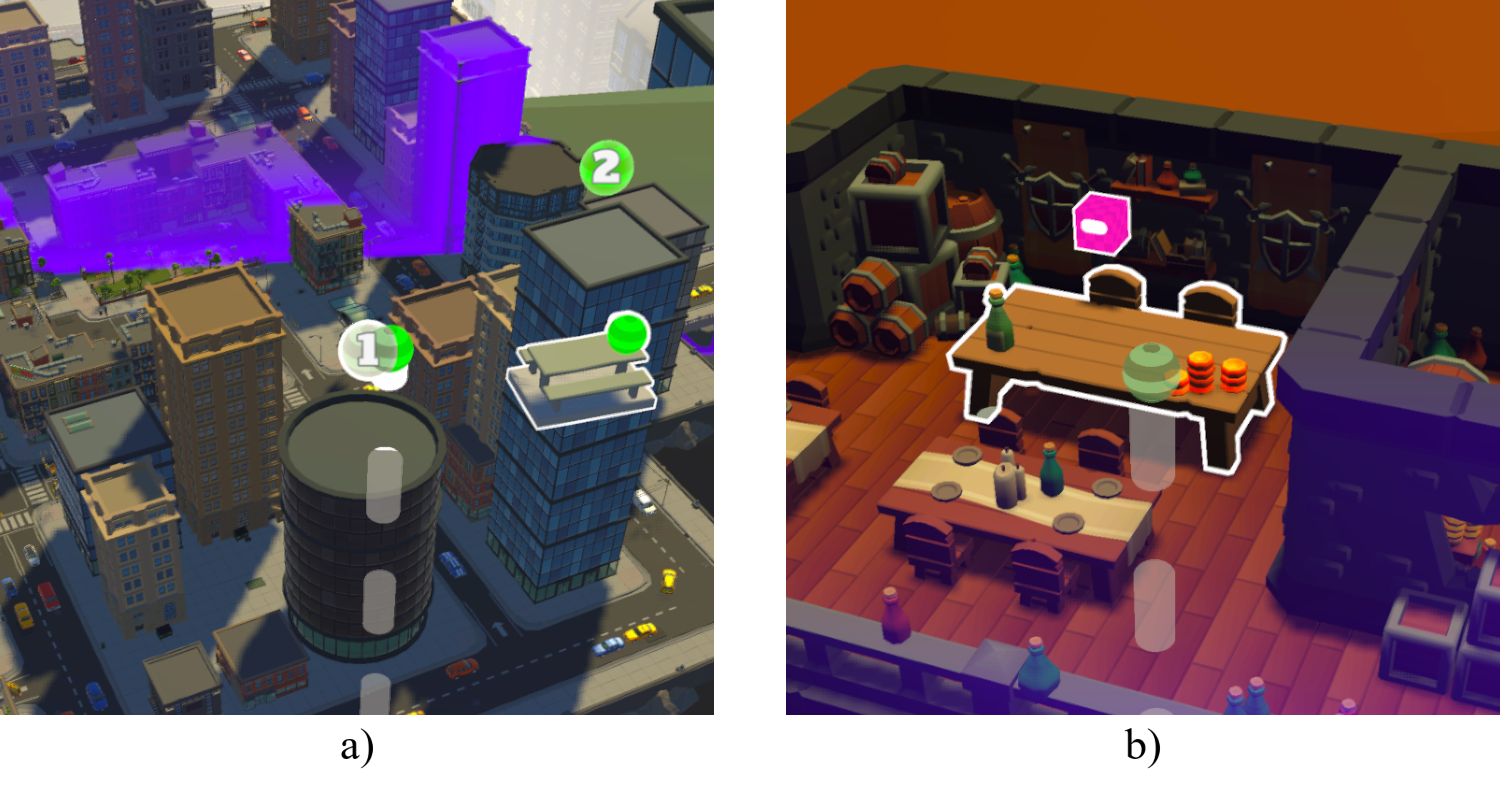
\includegraphics[width=1\textwidth]{figures/balloon_selection_intersection.png}
            \captionof{figure}{Balloon selection intersection with a point of interest in image a) and a table in image b).}
            \label{fig:balloon_selection_intersection}
        \end{figure}
    
\section{Networking}

    The prototype utilizes Unity's Netcode for GameObjects library to handle networking, enabling synchronization of GameObjects and Scenes across clients. This simplifies the management of the prototype's networking components. The networking architecture follows a client-server topology, illustrated in Figure \ref{fig:topology}. Specifically, it uses a client-hosted server named a host, where one client is also the server. This architecture was chosen for its simplicity in setup and management, and because it meets the prototype's requirements.

    \begin{figure}[h]
        \centering
        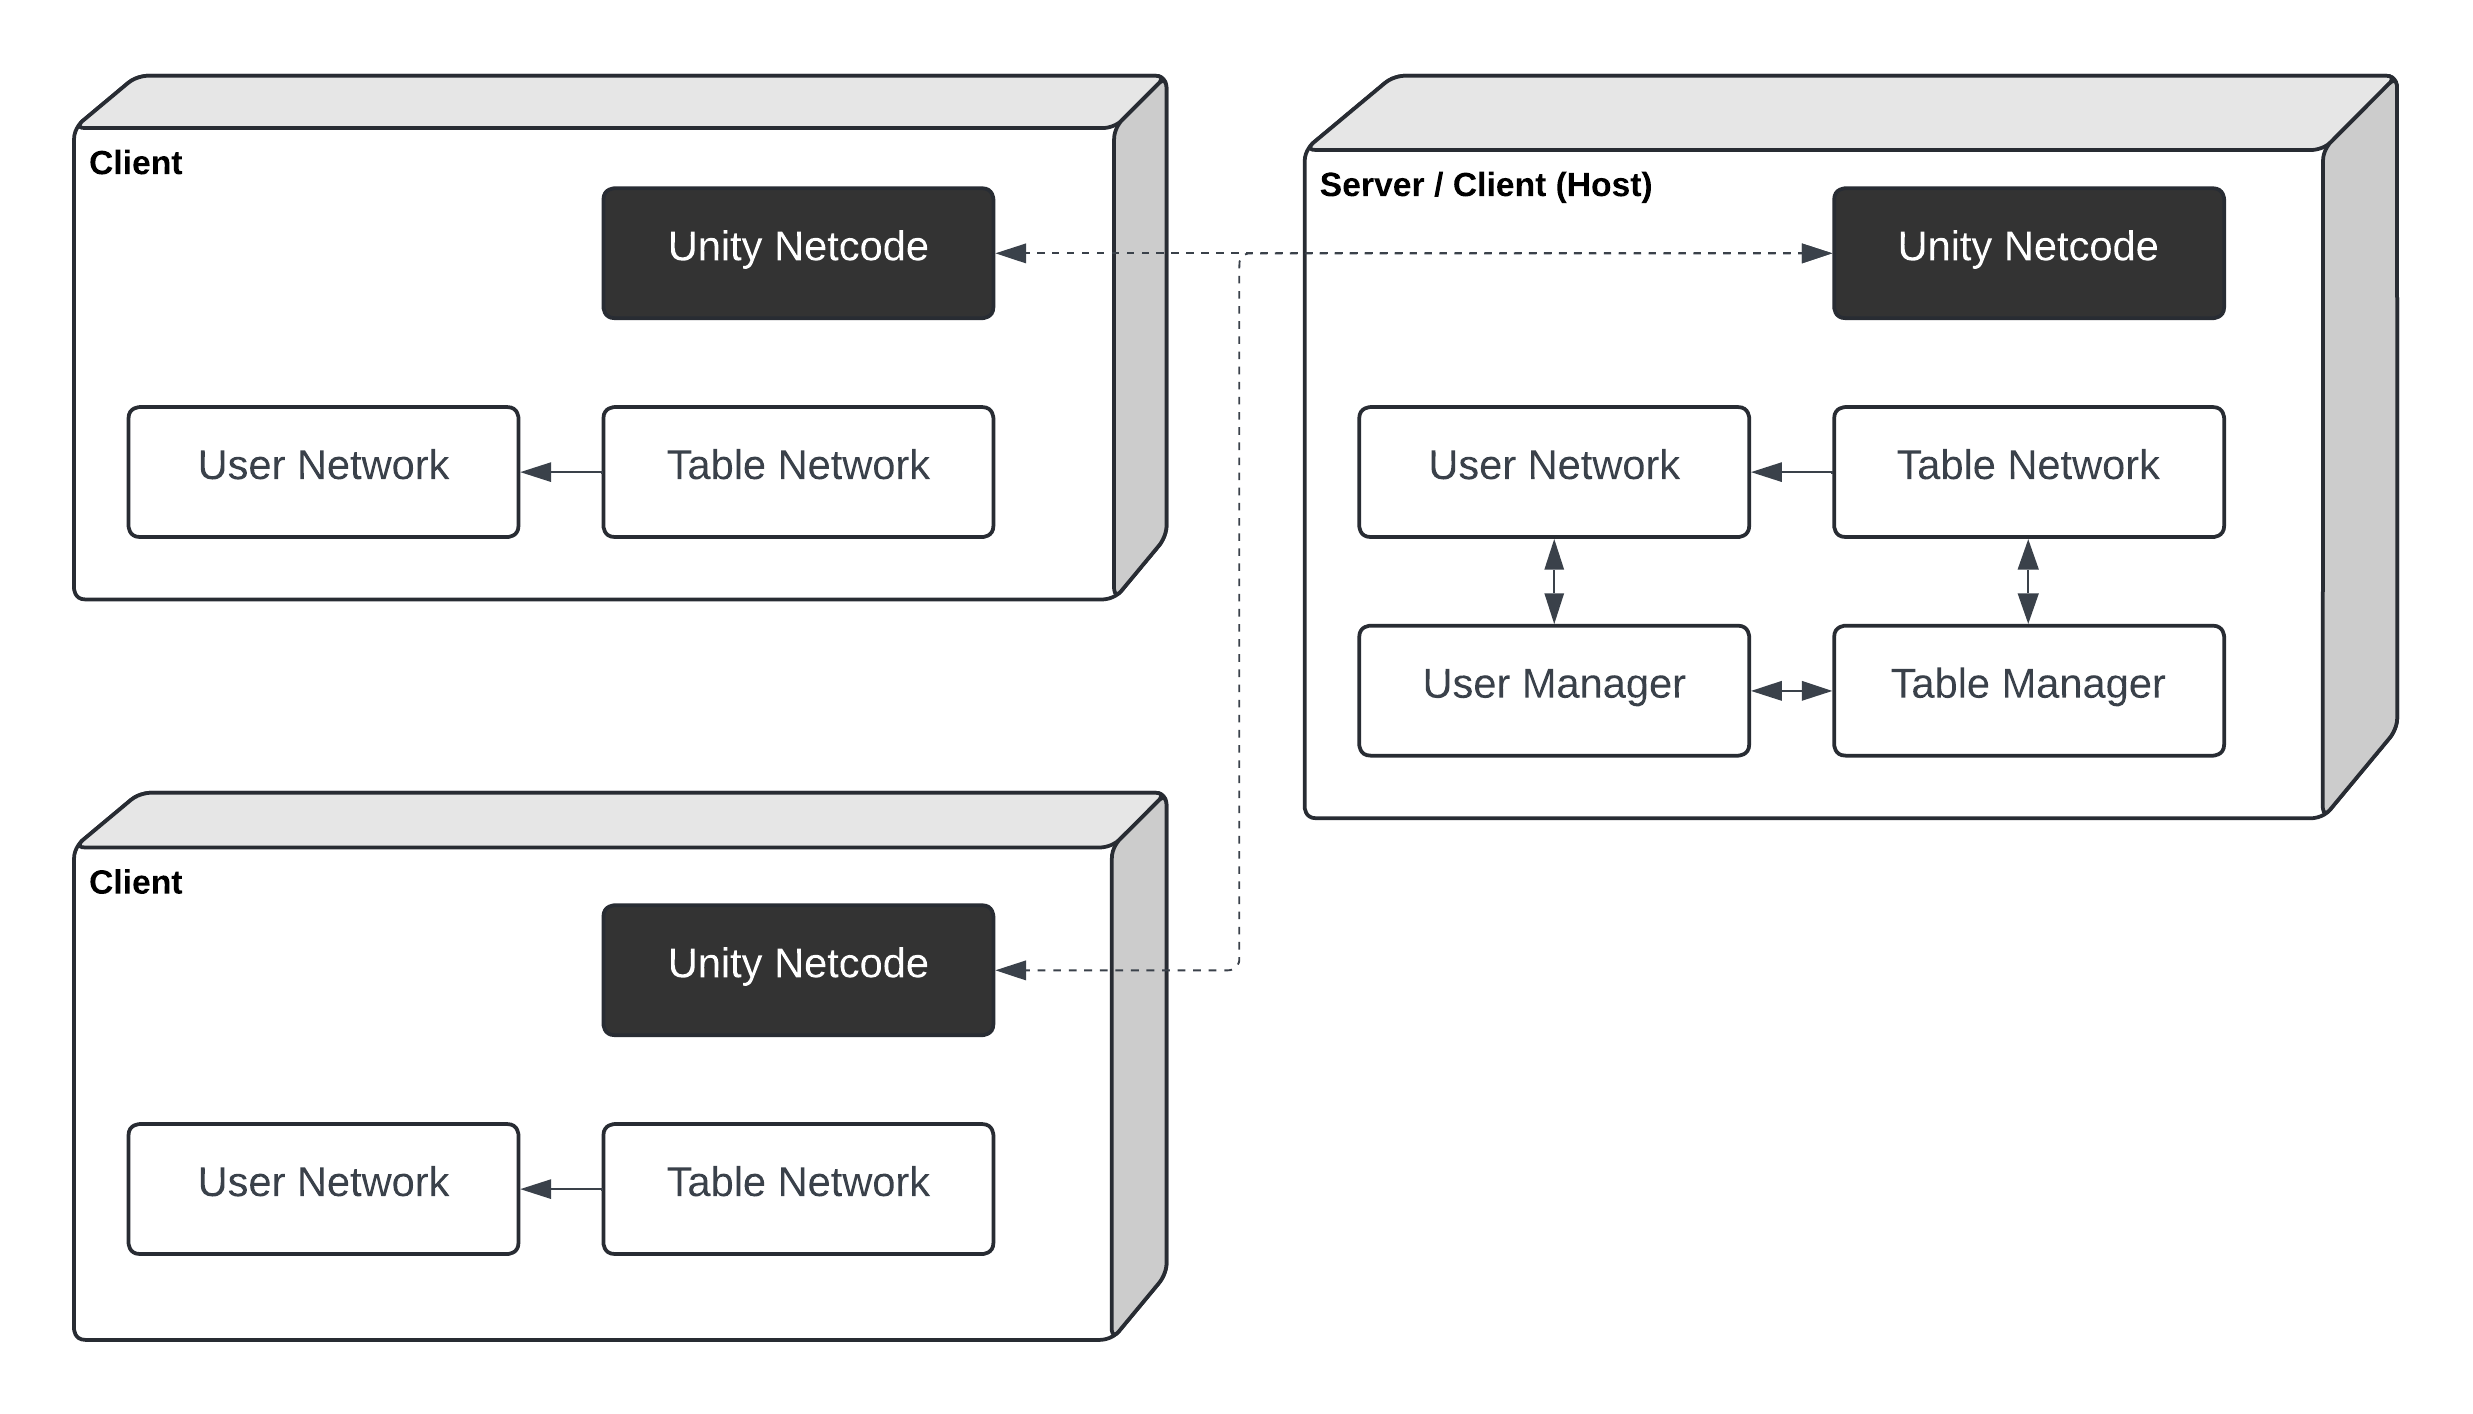
\includegraphics[width=.9\linewidth]{figures/topology.png}
        \caption{Networking architecture, using a client-server topology.}
        \label{fig:topology}
    \end{figure}

    Each client has a user network object for each connected user and a table network object for each table in the scene. A NetworkObject is a GameObject that interacts with Netcode. Before an instantiated NetworkObject is synchronized across clients, it must be spawned. In the client-server architecture, only the server has the authority to spawn and despawn NetworkObjects. By default, NetworkObjects are owned by the server and tied to its lifecycle. However, the user network objects are an exception. These are player NetworkObjects, that are automatically spawned by the server whenever a client connects, assigned to the client with ownership, and despawned when the client disconnects.\footnote{\url{https://docs-multiplayer.unity3d.com/netcode/current/basics/networkobject/}}


    NetworkObjects share data through network variables, synchronized with new clients when they join the server and with existing clients when the data changes. Network variables can have different permissions for reading and writing data. In a client-server architecture, the default setting is that the server has read-write permissions, while clients have read-only permissions.\footnote{\url{https://docs-multiplayer.unity3d.com/netcode/current/basics/networkvariable/}} Sections \ref{sec:user_network} and \ref{sec:table_network} describe the user and table network objects in detail. 

    The server manages the user and table network objects through the User Manager and Table Manager, respectively. These managers store data about connected users and tables, such as the association of user IDs to Netcode client IDs, the current point of interest ID, and the connected user IDs. They also handle the creation and destruction of network objects. Detailed functions of these managers are described in Sections \ref{sec:user_manager} and \ref{sec:table_manager}.

    The managers communicate with network objects through updates on network variables and remote procedure calls (RPCs). An RPC allows methods to be called on objects in another executable. In Netcode, RPCs execute methods on NetworkObjects across clients. A client can call an RPC on the server, and the server can call an RPC on a client. Clients can also call RPCs on other clients, though this passes through the server as a proxy.\footnote{\url{https://docs-multiplayer.unity3d.com/netcode/current/advanced-topics/message-system/rpc/}} Section \ref{sec:sequence_events} describes the sequence of events during the prototype's execution, including the RPCs used and other network-related events.

    \subsection{User Network Object} \label{sec:user_network}

        User network objects use network variables to store and synchronize data about the users. They have three network variables: user ID, a list of points of interest, and user transform data. The user ID identifies the user and determines their appearance. The list of points of interest contains the ID, position, and user ID of each point created by the user. The user transform data includes the user's position and rotation.

        The user ID and points of interest can only be modified by the server, while the user transform data is updated by the client. This design choice simplifies the synchronization of the table tracking algorithm described in Section \ref{sec:table_tracking}. The server assigns the user ID when the user joins, and updates the points of interest list as the user creates or removes points. The client updates the user transform data whenever the user moves.
        
        When a user network object receives an update to the user ID it updates the user's appearance. If the client owns the user network object, it also updates the balloon's appearance of the balloon selection.

        When a user creates a point of interest, a temporary point of interest is first created on the client, without an identification number, in both the replica and the 3D model. The temporary point of interest's position and user ID are sent to the user manager through an RPC. The user manager assigns an identification number to the point of interest and updates the appropriate user network object's points of interest list. Whenever this list is updated, the user network objects determine the type of update. If the client is the owner of the user network object and a point has been added, the temporary point of interest is updated with the identification number. If the client is not the owner, the replica controller is updated with the new point of interest, and marks it as unacknowledged. If a point of interest is removed, the user network object removes the point of interest from the replica controller. Late-joining users acquire all the spawned user network objects and update the WIM with the points of interest. 

    \subsection{Table Network Object} \label{sec:table_network}

        Table network objects have three network variables: transform data, the user ID seated at the first seat, and the user ID seated at the second seat. The transform data includes the table's position and rotation. Only the server can modify these variables, managed by the table manager. When a table network object is spawned, clients create a table replica in the WIM with the defined transform and seat data. When the table is despawned, the table replica is destroyed. Late-joining users acquire all the spawned table network objects and create table replicas accordingly.

        When the server updates the table network object's transform data, clients update the local table instance and the table replica's transform data. If a client is seated at the table, the client moves to the new position using the tracking data, as described in Section \ref{sec:table_tracking}. When the server updates the table network object's seat data, clients update the table replica to reflect who is seated at each seat.

    \subsection{User Manager} \label{sec:user_manager}
    
        The user manager is responsible for tracking and communicating with connected users. It maintains the association of user IDs to Netcode client IDs, the current point of interest ID, and the list of connected user IDs. When a user connects, Netcode triggers the \lstinline{OnClientConnected} event on the user manager, which assigns a user ID and updates the list of connected user IDs. For this prototype, only two users can be connected, so the user manager has a list of available user IDs, 0 and 1, which it assigns to new users. After updating the user's ID network variable, the user manager requests the table manager to add the player to an available table, as described in Section \ref{sec:table_manager}. Once a table is assigned, the user manager sends a \lstinline{MoveUserToTableClientRpc} to the user network object to move the user to the table, as shown in Figures \ref{fig:connect_and_create} and \ref{fig:connect_and_join}. When a user disconnects, the user manager removes the user ID from the list of connected user IDs and adds it back to the list of available user IDs. It then requests the table manager to remove the player from their table, as depicted in Figure \ref{fig:disconnect}. The spawning and despawning of user network objects are handled automatically by Netcode.

        When a user creates a point of interest, the user's network object sends a \lstinline{CreatePointOf}\lstinline{InterestRpc} to the user manager. The user manager increments the current point of interest ID and updates the user network object's points of interest list. Because this list is a network variable, it is synchronized across all clients, and the user network object handles the update accordingly, as described in Section \ref{sec:user_network}. When a user removes a point of interest, the user network object sends a \lstinline{RemovePointOfInterestRpc} to the user manager. The user manager then removes the point of interest from the network object's list.
        
        When a user teleports or joins a table, the user network object sends a \lstinline{MoveUserTo}\lstinline{PositionRpc} or \lstinline{MoveUserToTableRpc} to the user manager. The user manager then instructs the table manager to move the user to the new position or table, as outlined in Section \ref{sec:table_manager}. Afterward, the user manager sends a \lstinline{MoveUserToTableClientRpc} to update the user network object's position, as illustrated in Figures \ref{fig:teleport} and \ref{fig:table_join}.

    \subsection{Table Manager} \label{sec:table_manager}

        The table manager oversees the table network objects and assigns users to tables. Its primary functions include assigning newly connected users to available tables, managing user teleportation, handling users joining tables, and removing users from tables upon disconnection.

        When assigning a user to a table, the table manager first checks for available seats at existing tables. If a seat is available, the user is assigned to it. If no seats are available, the table manager creates a new table and assigns the user to the first seat. These scenarios are depicted in Figures \ref{fig:connect_and_create} and \ref{fig:connect_and_join}. When a user disconnects, the table manager removes them from their table. If the table becomes empty, it is despawned. This process is illustrated in Figure \ref{fig:disconnect}.

        When handling user teleportation, the table manager first checks if the user is alone at their current table. If they are, it moves the table to the new position. If the user is not alone, a new table is created at the new position, and the user is assigned to the first seat. These scenarios are depicted in Figure \ref{fig:teleport}.

        When a user joins a table, the table manager removes them from their original table. If the original table becomes empty, it is despawned. The user is then assigned to the first available seat on the new table. This process is shown in Figure \ref{fig:table_join}.


    \subsection{Sequence of Events} \label{sec:sequence_events}

        This section outlines a typical scenario that demonstrates the key interactions between users, tables, and the network. The diagrams illustrated only show the interaction between one client and the server at a time, from the perspective of the owner of the depicted user network object. Whenever a network variable is updated, the change is synchronized across all clients.

        The scenario begins with a user creating a server, thereby becoming its host. In this case, RPCs are local and executed instantly since the server also functions as a client. The client then connects to the server, as shown in Figure \ref{fig:connect_and_create}. The user manager assigns the user the ID 0 by updating the user's network variable and the list of connected user IDs. Upon updating this ID, the user's model is updated to the correct appearance. The user manager then requests the table manager to assign the user to an available table. Since no other users are connected, the table manager creates a new table, Table Network 1, and assigns the user to the first seat. When the table is spawned, it requests the local client to create the table replica on the WIM. The user manager then sends an RPC to the user network object, moving the user to the table.

        \begin{figure}[h]
            \centering
            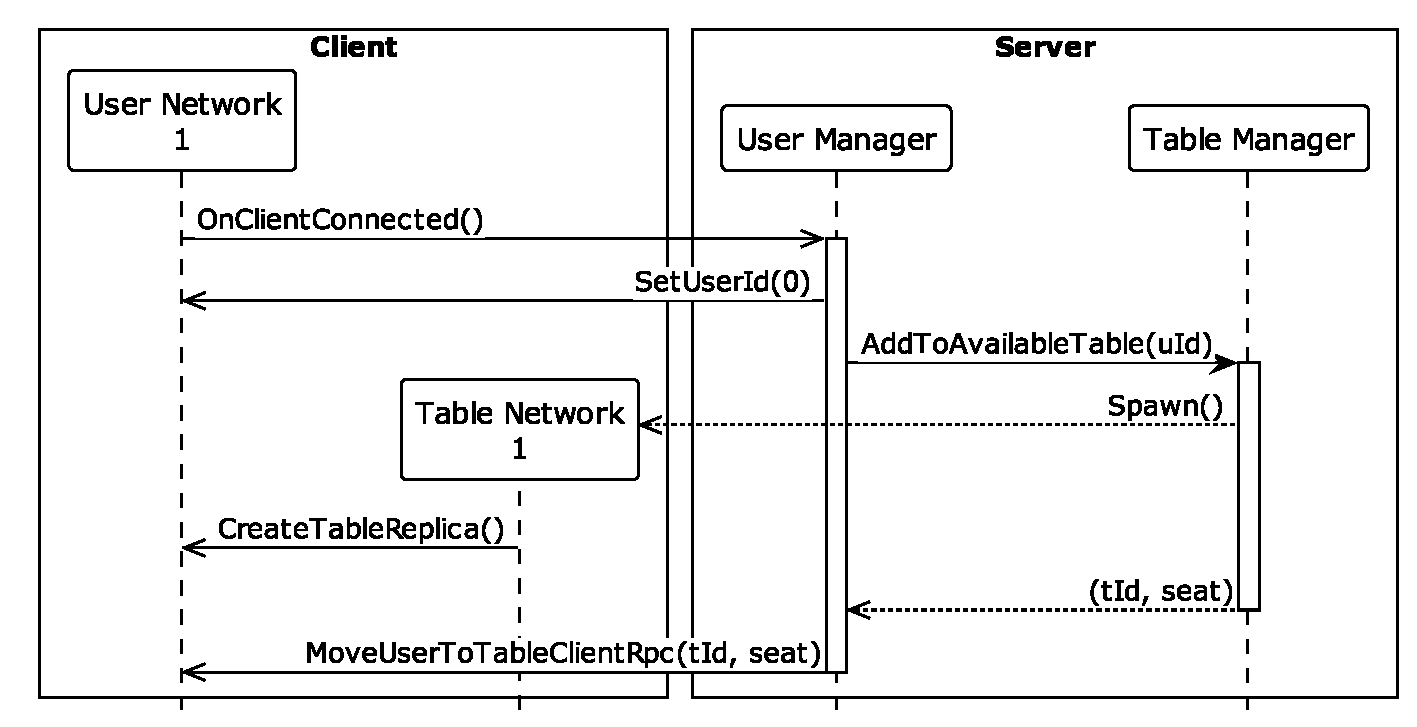
\includegraphics[width=.85\linewidth]{diagrams/out/connect_and_create_table.eps}
            \caption{Sequence diagram of a user connecting and creating a table.}
            \label{fig:connect_and_create}
        \end{figure}

        Next, the user creates a point of interest. Initially, a temporary point of interest is created on the client, followed by sending a \lstinline{CreatePointOfInterestRpc} to the user manager. The user manager increments the current point of interest ID and updates the user network's points of interest list. When the user network object receives this update, it assigns the identification number to the temporary point of interest, as it is owned by the client.

        The user then teleports to a new position, shown in Figure \ref{fig:teleport}. The user network object sends a \lstinline{MoveUserTo}\lstinline{PositionRpc} to the user manager, which instructs the table manager to move the user to the new location. Since the user is alone at the table, the table is moved to the new position, updating its network variables accordingly. The table network object, upon receiving these updates, adjusts the table replica on the client, and moves the user to the new position.

        \begin{figure}[h]
            \centering
            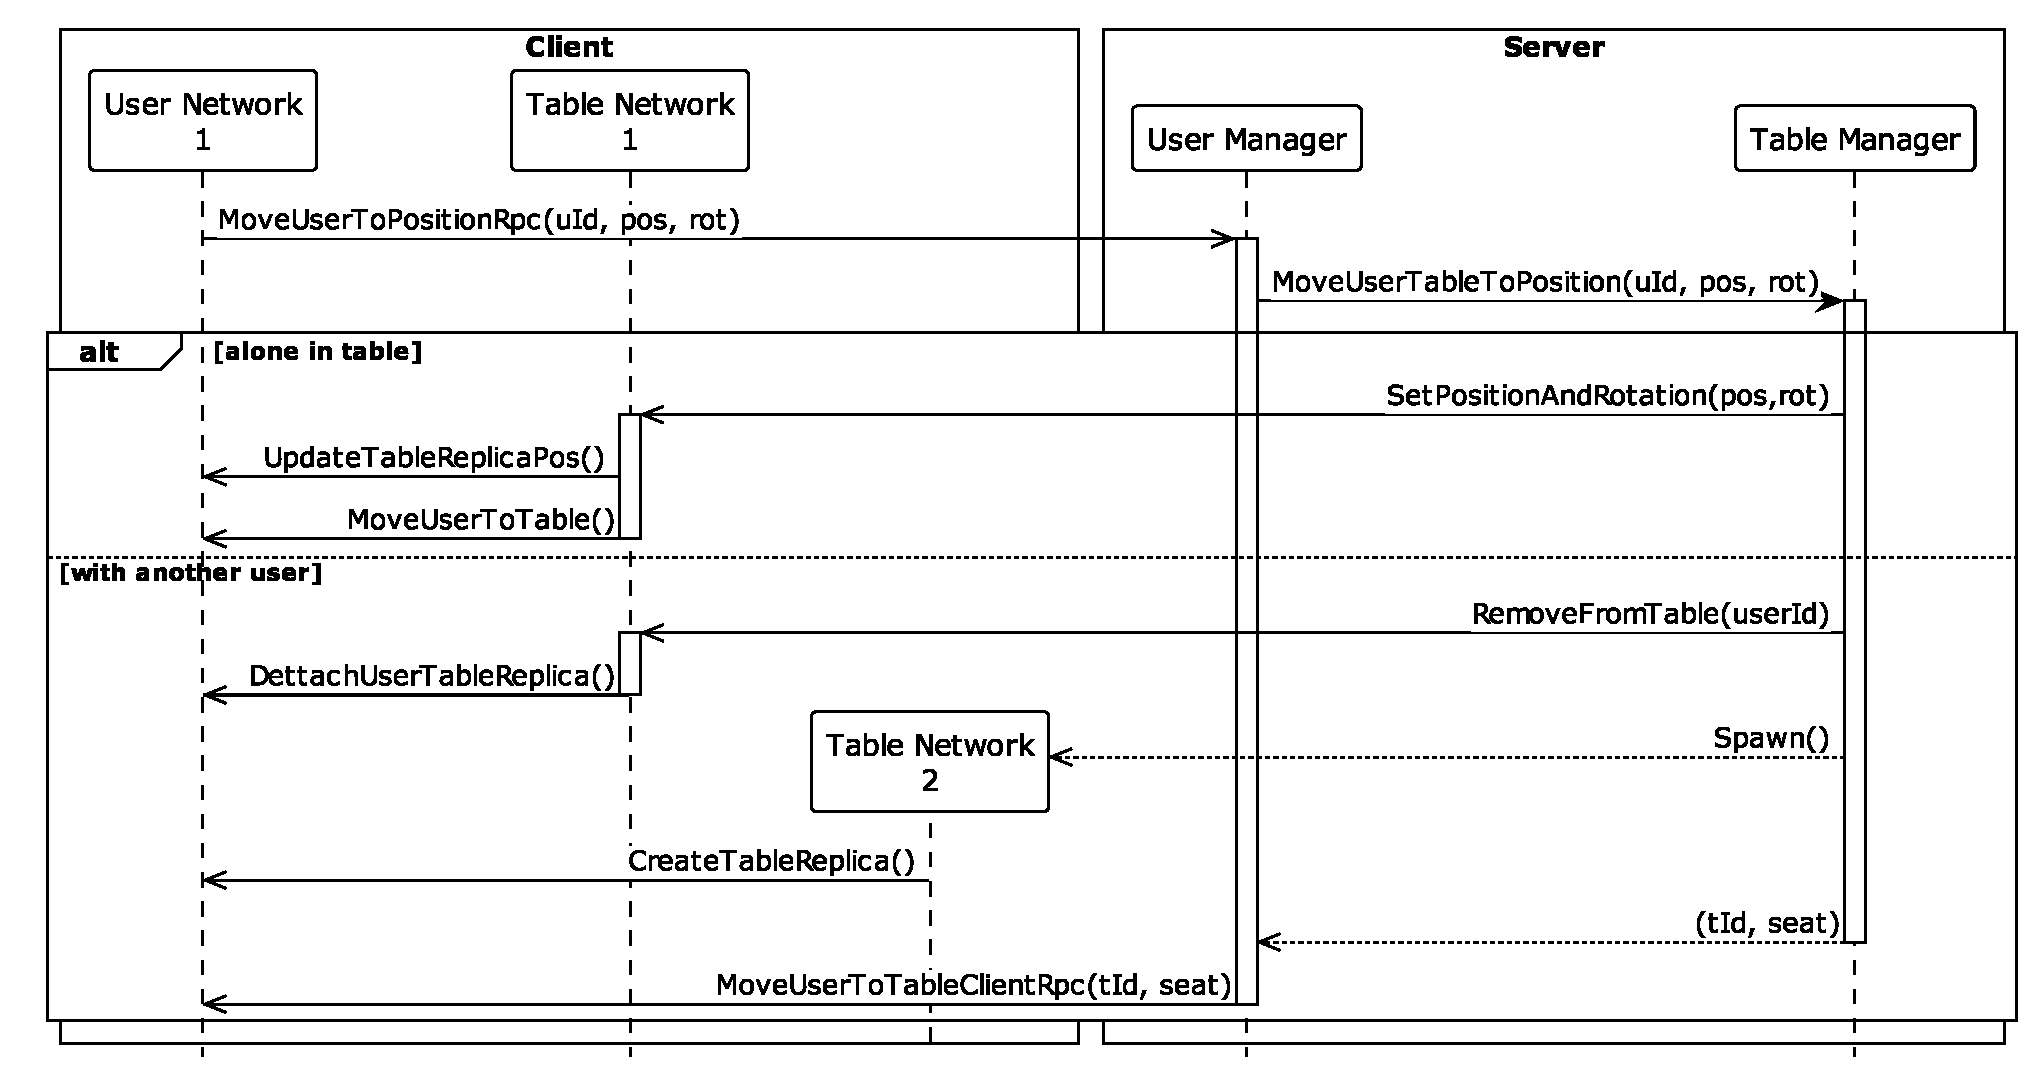
\includegraphics[width=.85\linewidth]{diagrams/out/teleport.eps}
            \caption{Sequence diagram of a user teleporting.}
            \label{fig:teleport}
        \end{figure}

        Later, another user connects to the server, as illustrated in Figure \ref{fig:connect_and_join}. The user manager assigns this user the ID 1 and updates the list of connected user IDs. Consequently, the user network object is updated with the new user ID and the corresponding appearance. The table manager assigns the new user to the second seat of Table Network 1, updating its seat network variables. The table network object then updates the table replica on each client, displaying the new user in the second seat. Following this, the user manager sends an RPC to the user network object to position the user at the table.

        \begin{figure}[ht!]
            \centering
            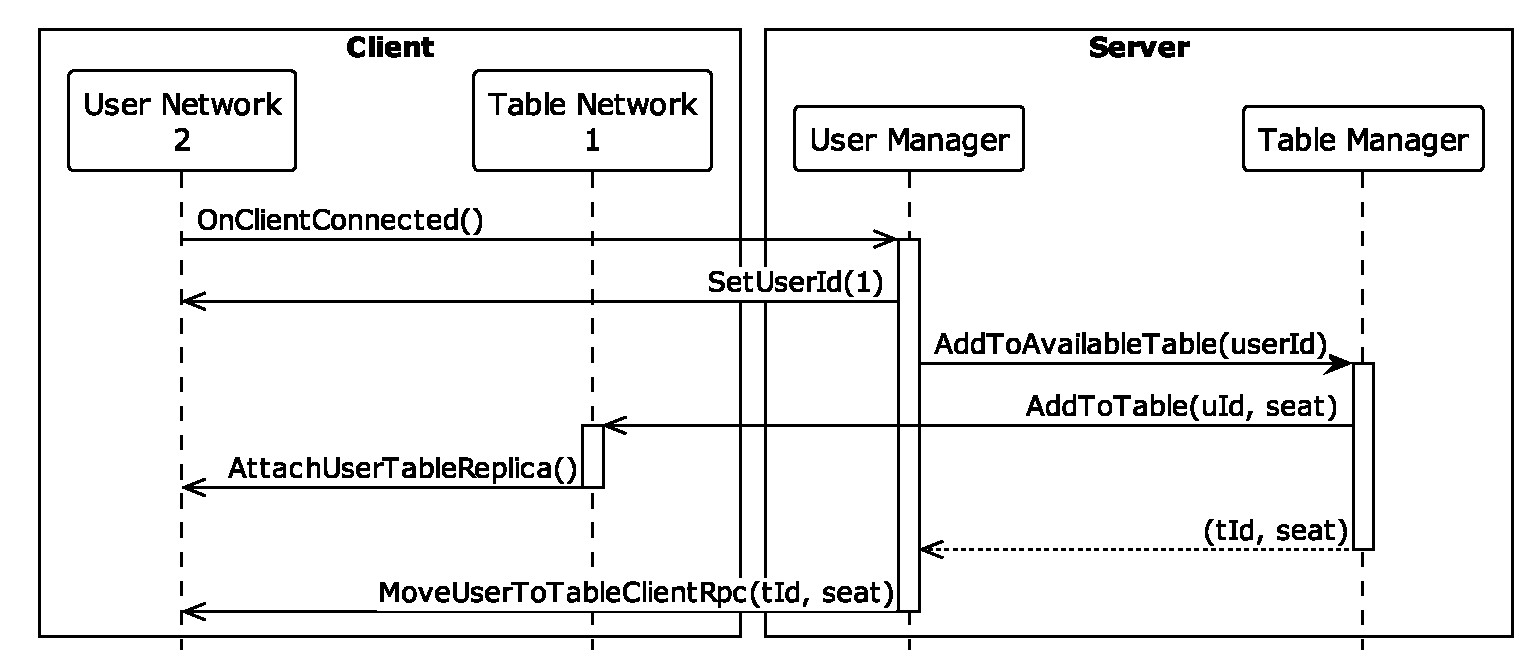
\includegraphics[width=.85\linewidth]{diagrams/out/connect_and_join_existing_table.eps}
            \caption{Sequence diagram of a user connecting and joining an existing table.}
            \label{fig:connect_and_join}
        \end{figure}

        Upon joining, the second user gathers information about the first user's points of interest by loading the point of interest data from the first user's network object, marking them as unacknowledged. Since acknowledgment data is local, no network communication is required. The second user would also load table data from other table network objects if any additional tables existed.

        Next, the first user moves to a new position, as depicted in Figure \ref{fig:teleport}. The user network object sends a \lstinline{MoveUserToPositionRpc} to the user manager, which instructs the table manager to relocate the user. Because the user is not alone at the table this time, the table manager removes the user from Table Network 1 and spawns a new table, Table Network 2, assigning the user to the first seat. The new table network object updates the table replica on each client to reflect the user's new position, while the old table network object removes the user from the replica. Finally, the user manager sends an RPC to the user network object, moving the user to the new table.

        Following this, the second user joins the second table, as shown in Figure \ref{fig:table_join}. Their network object sends a \lstinline{MoveUserToTableRpc} to the user manager, which instructs the table manager to move the user to the second table. The table manager removes the user from Table Network 1 and assigns them to the second seat of Table Network 2. Since Table Network 1 is now empty, it is despawned. The table network objects update the table replicas on each client accordingly. The user manager then sends an RPC to the user network object, positioning the user at the new table.
        
        \begin{figure}[h!]
            \centering
            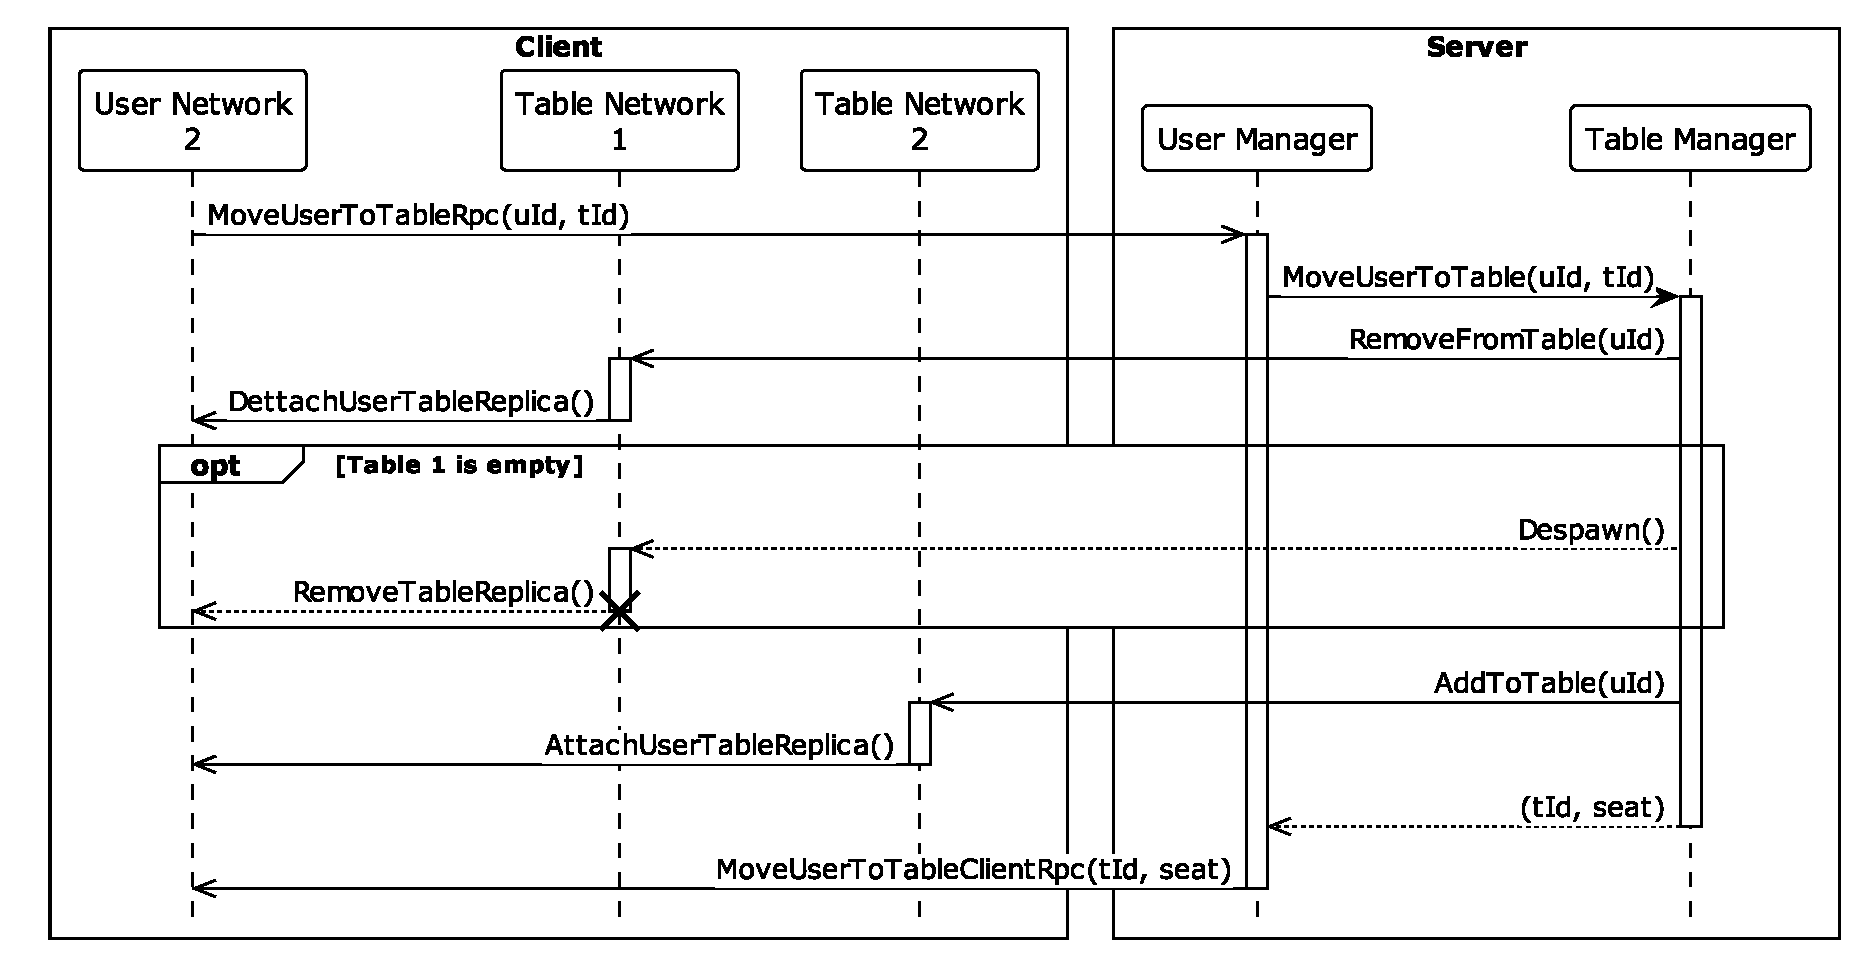
\includegraphics[width=.85\linewidth]{diagrams/out/table_join.eps}
            \caption{Sequence diagram of a user joining a table.}
            \label{fig:table_join}
        \end{figure}

        Finally, the first user disconnects, as depicted in Figure \ref{fig:disconnect}. The user manager removes the user ID from the list of connected user IDs and returns it to the list of available user IDs. It then instructs the table manager to remove the user from their table. The table network object updates the table replica on each client to reflect the user's removal. The user network object is automatically despawned by Netcode.

         \begin{figure}[h!]
            \centering
            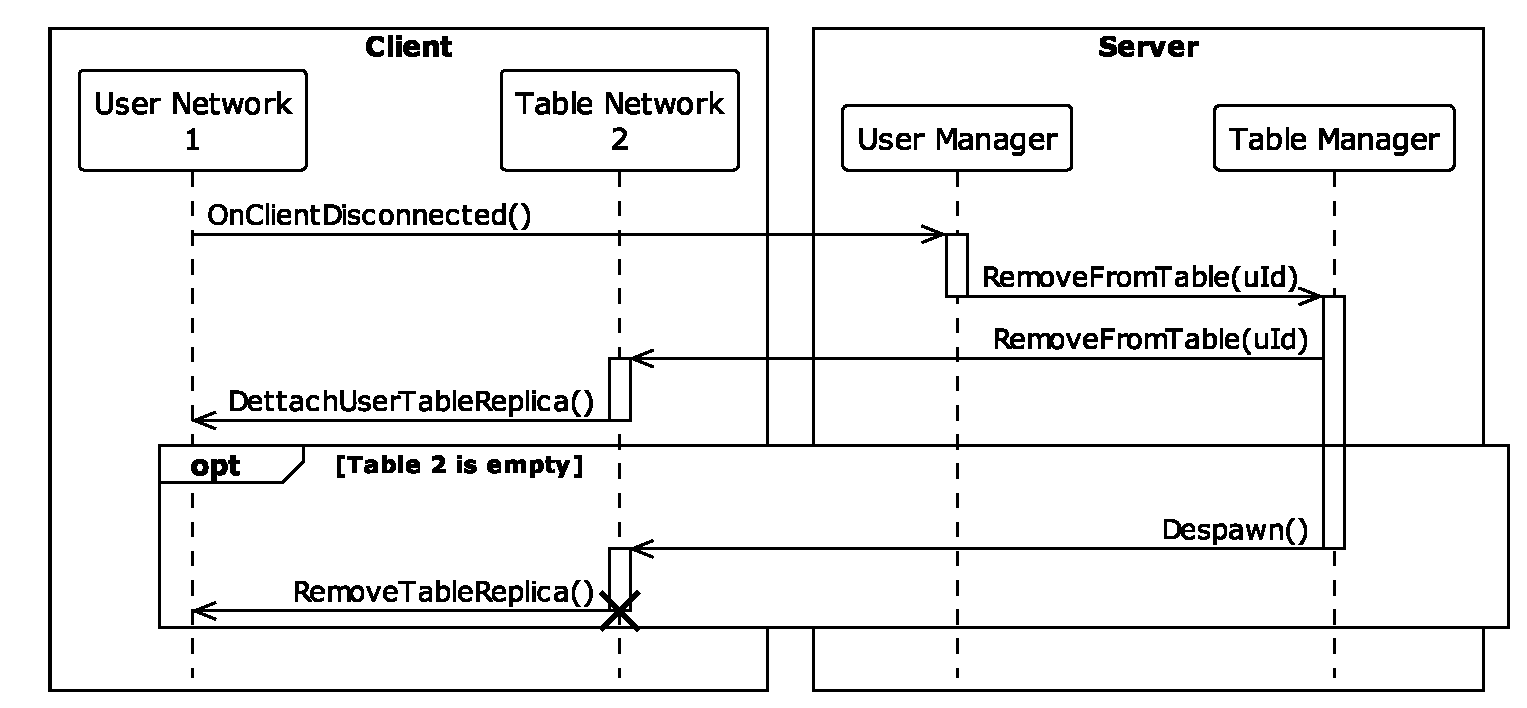
\includegraphics[width=.85\linewidth]{diagrams/out/disconnect.eps}
            \caption{Sequence diagram of a user disconnecting.}
            \label{fig:disconnect}
        \end{figure}

\section{Summary}
    This chapter details the implementation of a prototype for Replico. It starts with an overview of the system architecture and the hardware and software environment utilized, including Unity, Netcode for GameObjects, OpenXR, two HTC Vive Pro 2 headsets, and two multi-touch surfaces.

    The chapter continues by describing the state machine used to manage the prototype's states. These states range from the initial state, to \lstinline{TransformReplicaState} where users can manipulate the replica, and \lstinline{BalloonSelectionInitialState} where users can create, delete, and acknowledge points of interest, teleport, and join tables.

    Furthermore, the chapter details the calculations required to use the multi-touch input to transform the replica. Then, it details the gesture detection mechanisms used, including the utilization of the K-means clustering algorithm implemented via the ML.NET library for hand detection. Additionally, it outlines the use of VR controllers to track the user's interactions with virtual tables.

    The chapter describes the visual indicators implemented in the prototype. These include visual cues such as finger trails on the virtual touch frame, glow effects signaling gesture detection, illumination effects marking the touch frame's boundaries on the replica, and the visual representation of tables, table replicas, points of interest, and their corresponding visual appearances.

    The networking implementation is explained, describing the architecture, user and table network objects, user and table managers, network variables, and RPCs. The section ends with an outline of a typical sequence of events that unfold during the prototype's operation.
